\documentclass[]{scrartcl}

\usepackage{amsmath}
\usepackage{amssymb}
\usepackage[utf8]{inputenc}
\usepackage[T1]{fontenc}
\usepackage{lmodern}
\usepackage{ngerman}
\usepackage{geometry}
\usepackage{graphicx}
\usepackage{wrapfig}
\usepackage{caption}
\usepackage{wasysym}
\usepackage[separate-uncertainty = true,multi-part-units=single]{siunitx}
\usepackage{picinpar}
\usepackage{tikz}
\usepackage{float}
\usepackage{booktabs}

\renewcommand{\figurename}{Abb.}
\usepackage[
	colorlinks=true,
	urlcolor=blue,
	linkcolor=black
]{hyperref}


%Hier Titel und so
\newcommand{\versuchnummer}{V51} 
\newcommand{\versuchname}{Schaltungen mit Operationsverstärkern} 
\newcommand{\versuchdatum}{28.11.16} 


\title{Versuch \versuchnummer\\ \versuchname}
\subtitle{Physikalisches Fortgeschrittenenpraktikum}
\author{Robert Rauter und Björn Lindhauer}
\date{\versuchdatum} 
\begin{document}
\begin{titlepage}
{\large \versuchdatum}
\vspace{7cm}
\begin{center}
\textbf{\huge Versuch \versuchnummer:}\\
\vspace{0.5cm}
\textbf{\huge \versuchname}\\
\vspace{0.2cm}
\textbf{ Physikalisches Fortgeschrittenenpraktikum}\\
\vspace{9cm}

{\Large Robert Rauter \ \ \hspace{1.5cm} und \hspace{1.5cm} Björn Lindhauer}\\
{ \url{robert.rauter@tu-dortmund.de} \ \ \hspace{2cm} \url{bjoern.lindhauer@tu-dortmund.de}}
\end{center}
\end{titlepage}
\section{Einleitung}
Mithilfe von Operationsverstärkern sollen verschiedene Schaltungen realisiert werden, die z.B. als Signalgeneratoren genutzt werden können.

\section{Theoretische Grundlagen}
\subsection{Ideale Operationsverstärker}
Ein Operationsverstärker wird durch das Schaltsymbol \ref{fig:schaltsymbol_operationsverstaerker} repräsentiert und ist ein elektronisches Bauteil, dessen Ausgangsspannung
\begin{align}
 U_{\text{A}}=V\cdot \left( U_{\text{P}}-U_{\text{N}} \right)
\end{align}
ist, welche somit proportional zur Differenz an den beiden Eingängen ist.

Deswegen wir er auch als gleichstromgekoppelter Differenzverstärker bezeichnet.

\begin{figure}[H]
\centering
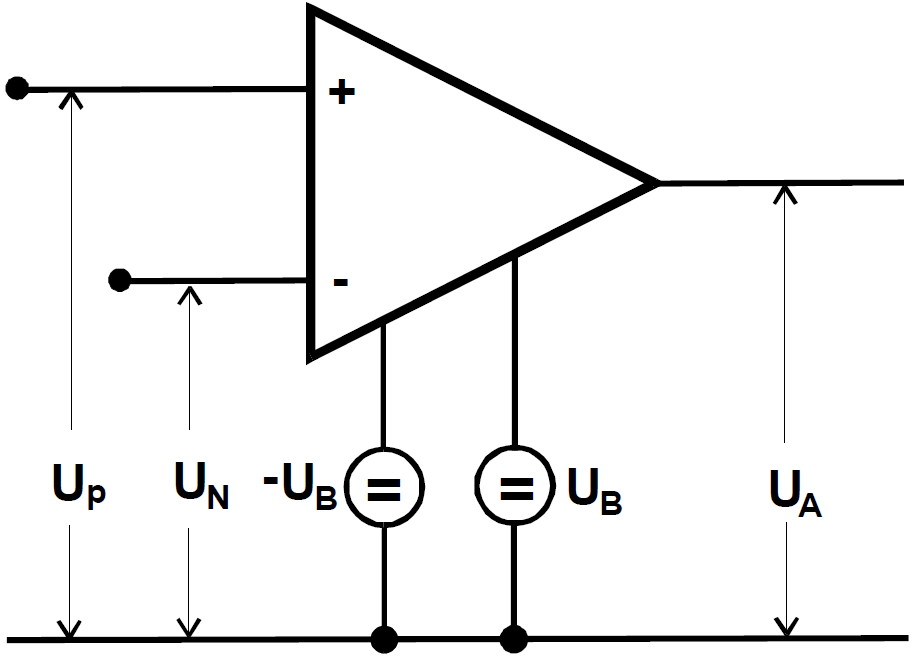
\includegraphics[width=7cm]{images/schaltsymbol_operationsverstaerker.png}
\caption{Schaltsymbol eines Operationsverstärkers. Die Betriebsspannung $\pm U_{\text{B}}$ wird jedoch häufig nicht mit eingezeichnet. [1]}
\label{fig:schaltsymbol_operationsverstaerker}
\end{figure}

Die Betriebsspannung $\pm U_{\text{B}}$ limitiert das Ausgangssignal $U_{\text{A}}$ auf dem Bereich
\begin{align}
 -U_{\text{B}} < U_{\text{A}} < U_{\text{B}}
\end{align}
und sorgt für eine Sättigung bei $\left| U_{\text{A}} \right| > U_{\text{B}}$. Der Verlauf der Kurve ist in Abbildung \ref{fig:kennlinie_operationsverstaerker} schematisch dargestellt. 

Es wird der Eingang mit der Spannung $U_{\text{P}}$ als nicht-invertierter Eingang (+) bezeichnet, da die Ausgangsspannung $U_{\text{A}}$ n Phase mit der Spannung $U_{\text{P}}$ ist.
Die Ausgangsspannung ist jedoch gegenphasig zur Spannung $U_{\text{N}}$, weshalb deren Eingang als invertierter Eingang (-) bezeichnet wird.

Bei einem idealen Operationsverstärker ist die Leerlaufverstärkung $V$, sowie der Eingangswiderstand $r_{e}$ unendlich groß und der Ausgangswirderstand $r_a$ verschwindet.

Dies ist beim realen Operationsverstärker jedoch nicht der Fall, sodass es sinnvoll ist, weitere Größen zu definieren.

\begin{figure}[H]
\centering
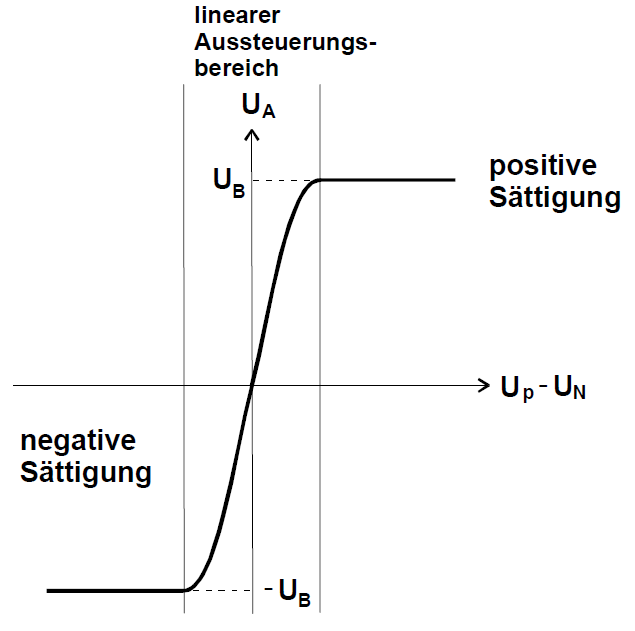
\includegraphics[width=7cm]{images/kennlinie_operationsverstaerker.png}
\caption{Kennlinie eines Operationsverstärkers. Die Steigung der Geraden zwischen den Sättigungen ist in Realität wesentlich steiler. [1]}
\label{fig:kennlinie_operationsverstaerker}
\end{figure}

\subsection{Reale Operationsverstärker}
Die Ausgangsspannung ist von Null verschieden, wenn die beiden Eingangsspannungen gleich sind. Deshalb wird die Gleichtaktverstärkung
\begin{align}
 V_{gl}:=\frac{\Delta U_{A}}{\Delta U_{gl}}
\end{align}
definiert.

Aus den endlichen Eingangswiderständen folgen Eingangsruheströme $I_{P}$ und $I_{N}$, die zur Definition des Eingangsruhestroms
\begin{align}
 I_{B}:=\frac{1}{2} \cdot \left(I_{P}+I_{N}\right)
\end{align}
und des Offsetstroms
\begin{align}
 I_{0}:= \left. I_{P}-I_{N}\right|_{U_{P}=U_{N}=0} 
\end{align}
führen.

Der Differenzwiderstand wird als
\begin{align}
 r_{D}:=\left\lbrace 
\begin{array}{ll}
\frac{\Delta U_{P}}{\Delta I_{P}} & \text{, }U_{N}=0 \vspace{0.2cm}\\
\frac{\Delta U_{N}}{\Delta I_{N}} & \text{, }U_{P}=0
\end{array}
\right\rbrace 
\end{align}
definiert und der Gleichtakteingangswiderstand als
\begin{align}
 r_{gl}:=\frac{\Delta U_{gl}}{\Delta I_{gl}} \hspace{0.3cm}\text{.}
\end{align}

Da die Ausgangsspannung $U_{a}$ bei realen Operationsverstärkern ungleich null ist, wird die Offsetspannung
\begin{align}
 U_0:=\left. U_{P}-U_{N} \right|_{U_{a}=0}
\end{align}
definiert.

Diese ist häufig eine Funktion der Temperatur, Zeit und Betriebsspannung. Die totale Ableitung von $U_{0}$ wird Offsetspannungsdrift genannt.

Reale Operationsverstärker kommen idealen Operationsverstärkern sehr nahe, sodass die eingeführten Größen als Störparameter angesehen werden können und somit zu Korrekturen führen.

\subsection{Schaltungen mit Operationsverstärker}
In diesen Abschnitt sollen einige gängige Schaltungen mit Operationsverstärkern vorgestellt werden und ein paar grundsätzliche Eigenschaften der Schaltungen diskutiert werden.
\subsubsection{Linearverstärker}
Da ein Operationsverstärker bereits eine hohe Leerlaufverstärkung besitzt, ist der Ansteuerungsbereich gering und schon kleine Eingangsspannungen führen zu einer Sättigung.
\begin{figure}[H]
\centering
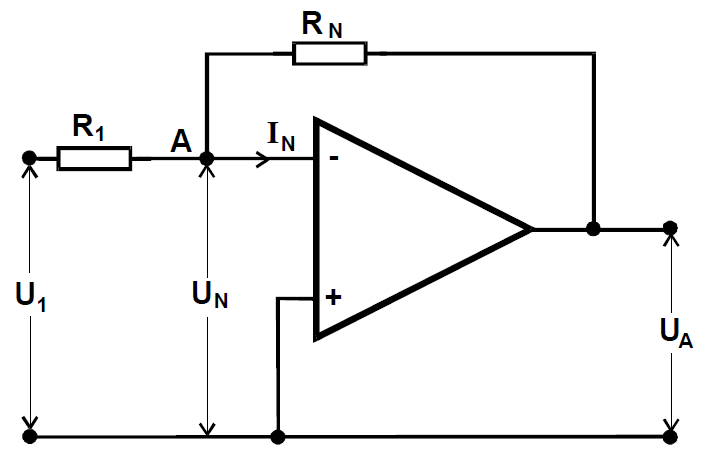
\includegraphics[width=9cm]{images/schaltplan_linearverstaerker.png}
\caption{Schaltplan eines gegengekoppelten invertierten Linearverstärkers. [1]}
\label{fig:schaltplan_linearverstaerker}
\end{figure}
Um dies zu unterbinden und höhere Eingangsspannungen zu verwirklichen, muss ein Gegenkopplungszweig, wie in Abbildung \ref{fig:schaltplan_linearverstaerker} integriert werden.

Es wird im Gegenkopplungszweig ein durch das Widerstandsverhältnis der eingebauten Widerstände bestimmter Anteil der Ausgangsspannung zurück auf den invertierten Eingang gegeben. Somit führt eine Zunahme der Ausgangsspannung zu einer Abnahme der Eingangsspannung.

Dies führt zwar zu einer Ausweitung des Ansteuerungsbereich, verringert jedoch die Gesamtverstärkung.

Die Verstärkung $V'$ ist in erster Ordnung nur vom Verhältnis der Widerstände
\begin{align}
V'=-\frac{R_{\text{N}}}{R_{1}}
\label{eq:verstaerkung_ideal}
\end{align}
abhängig.

Die Leerlaufspannung führt zu der Korrektur Verstärkung
\begin{align}
\frac{1}{V'}\approx \frac{1}{V} + \frac{R_{1}}{R_{\text{N}}}
\end{align}
für große Leerlaufspannungen $V \gg 1$. Die Gleichung \ref{eq:verstaerkung_ideal} ist folglich für $\frac{R_{\text{N}}}{R_{1}} \gg 1$ korrekt.

Wird eine solche starke Gegenkopplung verwirklicht, so haben thermische Fluktuationen der Leerlaufspannung nur einen kleinen Effekt auf die Schaltung, was die Stabilität der Schaltung verbessert.

Es werden durch die Gegenkopplung auch weitere Parameter positiv beeinflusst. So nimmt beispielsweise der endliche Ausgangswiderstand um den Faktor
\begin{align}
g:=\frac{V}{V'}
\end{align}
ab. Auch Schwankungen der Leerlaufverstärkung werden um den Faktor $g$ vermindert:
\begin{align}
\frac{\Delta V'}{V'}=g^{-1}\frac{\Delta V}{V}
\end{align}
Außerdem kann eine Größere Frequenzbrandbreite unverzerrt übertragen werden, da diese auch um den Faktor $g$ erhöht wird. In Abbildung \ref{fig:frequenzgang_operationsverstaerker} wird der Unterschied der Brandbreiten im Frequenzgang des Linearverstärkers dargestellt.
\begin{figure}[H]
\centering
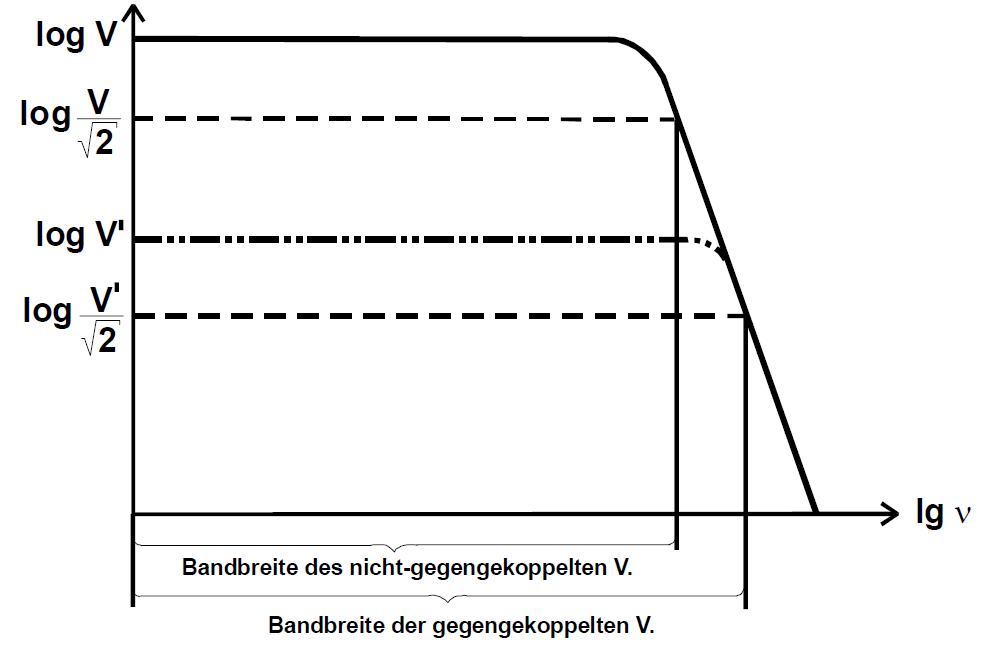
\includegraphics[width=9cm]{images/frequenzgang_operationsverstaerker.png}
\caption{Frequenzgang des Linearverstärkers. [1]}
\label{fig:frequenzgang_operationsverstaerker}
\end{figure}

Der geringe Eingangswiderstand der Schaltung nach Abbildung \ref{fig:schaltplan_linearverstaerker} ist in manchen Anwendungen, wie Messungen an hochohmigen Spannungsquellen, unvorteilhaft.

In diesen Fällen kann ein sogenannter Elektrometerverstärker nach Abbildung \ref{fig:schaltplan_elektrometerverstaerker} verwendet werden, der zwar auch invertierend gegengekoppelt ist, jedoch liegt die Eingangsspannung $U_1$ an den nicht-invertierten Eingang an. 

Dies führt zu einem Eingangswiderstand $r_\text{e}=\infty$ bei idealen Operationsverstärkern und $r_\text{e}\approx 2r_{\text{gl}}$ für einen realen Operationsverstärker, wobei $r_{\text{gl}}$ der Gleichtakteingangswiderstand ist und typischerweise in der Größenordnung von 20G$\Omega$ liegt.
\begin{figure}[H]
\centering
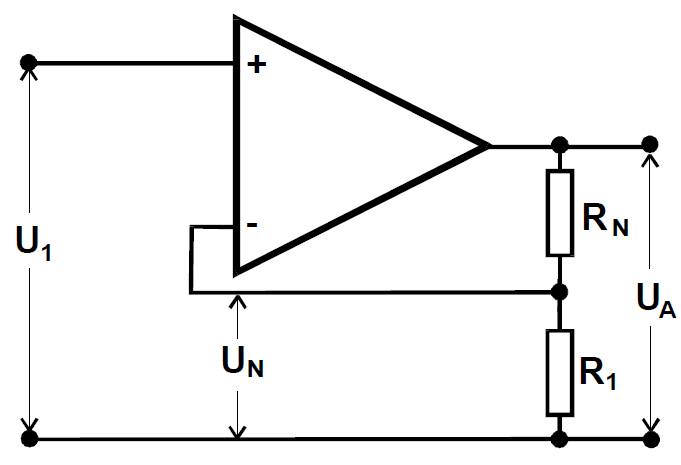
\includegraphics[width=9cm]{images/schaltplan_elektrometerverstaerker.png}
\caption{Schaltplan eines Elektrometerverstärkers. [1]}
\label{fig:schaltplan_elektrometerverstaerker}
\end{figure}
Es ergibt sich eine Verstärkung
\begin{align}
V'=\frac{R_\text{N}+R_1}{R_1}
\end{align}
des Elektrometerverstärkers bei idealen Operationsverstärkern.

Sollen kleine Ströme ohne großen Spannungsabfall gemessen werden, so wird ein Linearverstärker mit sehr geringem Eingangswiderstand $r_\text{e}$ benötigt. 

Der in Abbildung \ref{fig:schaltplan_linearverstaerker} dargestellte Linearverstärker besitzt in erster Ordnung den Eingangswiderstand $R_1$. Es liegt daher nahe, den Eingangswiderstand zu $R_1=0$ wählen. Ein solches Amp$\grave{\text{e}}$remeter ist in Abbildung \ref{fig:schaltplan_amperemeter} dargestellt.

Die Ausgangsspannung 
\begin{align}
U_\text{A}=IR_\text{N}
\end{align}
ist proportional zum Messstrom. Die Schaltung eignet sich somit zur Strommessung.
\begin{figure}[H]
\centering
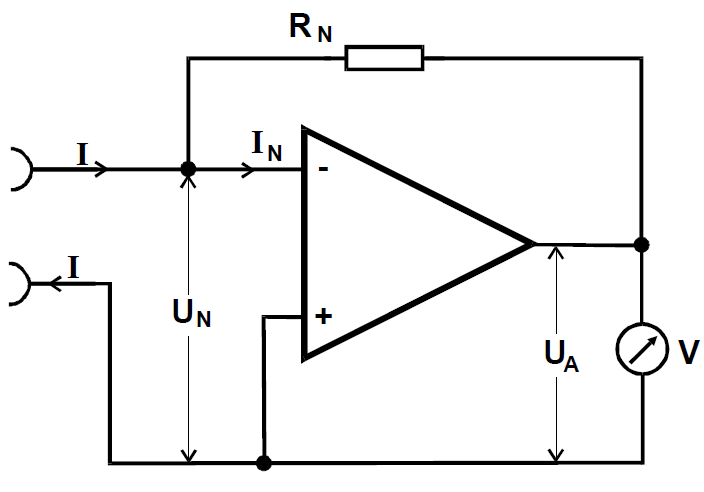
\includegraphics[width=9cm]{images/schaltplan_amperemeter.png}
\caption{Schaltplan eines Amp$\grave{\text{e}}$remeters}
\label{fig:schaltplan_amperemeter}
\end{figure}
\subsubsection{Umkehr-Integrator}
Wird ein Kondensator im Rückkopplungszweig eingebaut, wie in Abbildung \ref{fig:schalplan_umkehrintegrator}, so fungiert die Schaltung als Umkehr-Integrator
\begin{align}
U_\text{A}= \frac{1}{RC}\int dt\ U_1\left(t\right)  \hspace{0.3cm}\text{.}
\end{align}
\begin{figure}[H]
\centering
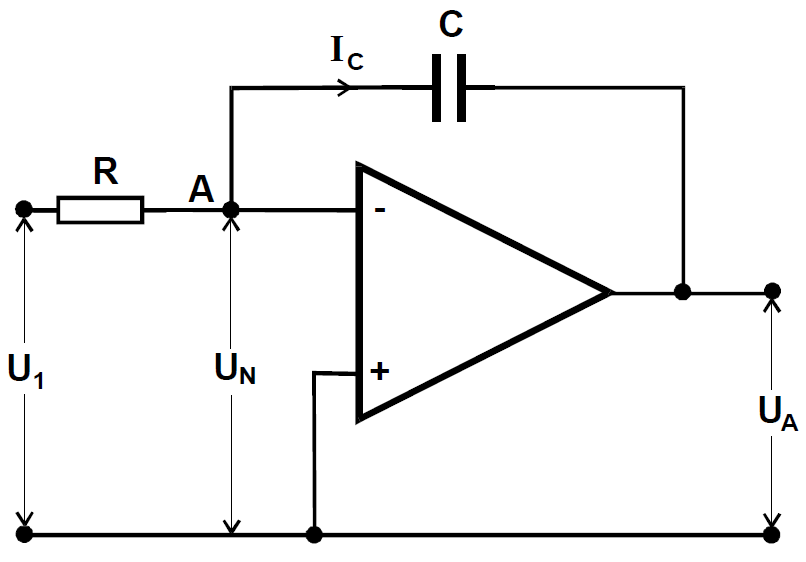
\includegraphics[width=9cm]{images/schalplan_umkehrintegrator.png}
\caption{Schaltplan eines Umkehr-Integrators. [1]}
\label{fig:schalplan_umkehrintegrator}
\end{figure}
Wird beispielsweise eine Sinusspannung an 
\begin{align}
U_1=U_0 \sin \omega t
\end{align}
angelegt, so hat das Ausgangssignal die Form
\begin{align}
U_\text{A} = \frac{U_0}{RC\omega}\cos \omega t
\end{align}
und ist umgekehrt proportional zur Frequenz des Eingangssignals.
\subsubsection{Umkehr-Differentiator}
Wird der Kondensator anstatt im Rückkopplungszweig vor den invertierten Eingang geschaltet, wie in Abbildung \ref{fig:schalplan_umkehrdifferentiator}, so wirkt die Schaltung als Umkehr-Differentiator
\begin{align}
U_\text{A}= -RC \frac{d}{d t} U_1 \hspace{0.3cm}\text{.}
\end{align}
\begin{figure}[H]
\centering
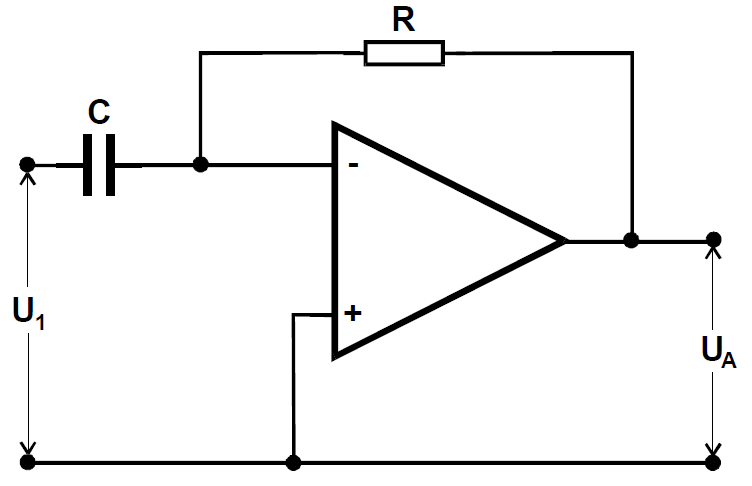
\includegraphics[width=9cm]{images/schaltplan_umkehrdifferentiator.png}
\caption{Schaltplan eines Umkehr-Differentiator. [1]}
\label{fig:schalplan_umkehrdifferentiator}
\end{figure}
Bei einer Sinusspannung
\begin{align}
U_1=U_0 \sin \omega t
\end{align}
kann am Ausgang die Spannung
\begin{align}
U_\text{A} = -RC\omega U_0 \cos \omega t
\end{align}
abgegriffen werden, welche proportional zur Frequenz des Eingangssignals ist.
\subsubsection{Schmitt-Trigger}
Bei einem Schmitt-Trigger wird bei einem gegengekoppelten invertierenden Linearverstärker die Rückkopplung anstatt am invertierenden Eingang auf den nicht-invertierenden Eingang gegeben. Diese Schaltung nach Abbildung \ref{fig:schalplan_schmitt_trigger} fungiert als ein Schalter.

Eine Vergrößerung der Ausgangsspannung führt beim Schmitt-Trigger zu einer Vergrößerung der Eingangsspannung, welche wiederum zu einer Vergrößerung der Ausgangsspannung führt. Diese Schaltung ist instabil, da die Ausgangsspannung spontan auf die Betriebsspannung $U_\text{B}$ springt, wenn die Spannung $U_1$ den Schwellwert
\begin{align}
\frac{R_1}{R_\text{P}}U_\text{B}
\end{align} 
überschreitet. Umgekehrt springt die Ausgangsspannung auf die negative Betriebsspannung $-U_\text{B}$, wenn der Schwellwert
\begin{align}
-\frac{R_1}{R_\text{P}}U_\text{B}
\end{align}
unterschritten wird.

Die Differenz der beiden Umschaltwerte wird als Schalthysterese bezeichnet.
\begin{figure}[H]
\centering
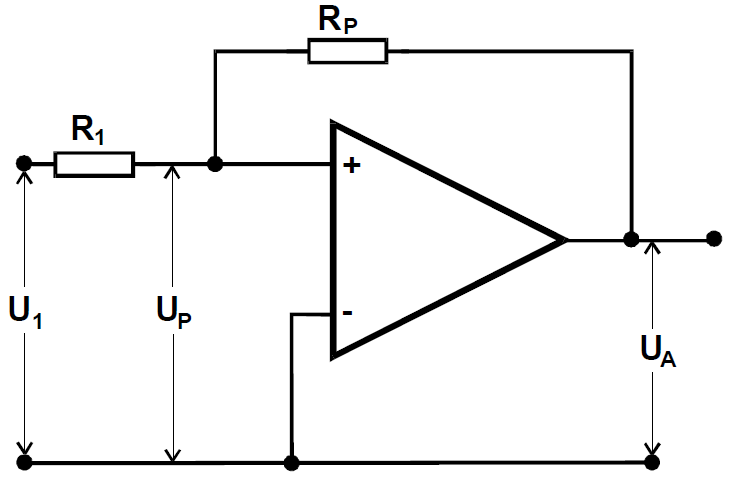
\includegraphics[width=9cm]{images/schaltplan_schmitt_trigger.png}
\caption{Schaltplan eines Schmitt-Triggers. [1]}
\label{fig:schalplan_schmitt_trigger}
\end{figure}


\subsubsection{Der Operationsverstärker als Signalgenerator}
Mit Hilfe der in den vorherigen Abschnitten beschriebenen Schaltungen lässt sich ein Rechteck- und Dreiecksgenerator erzeugen. 

Es wird dabei jeweils ein Schmitt-Trigger und ein Integrator benötigt, die wie in Abbildung \ref{fig:schalplan_generator} geschaltet werden.

Der Schmitt-Trigger liefert eine konstante Ausgangsspannung $U_\text{B}$, die anschließend vom Integrator integriert wird. Es fällt somit die Ausgangsspannung $U_1$ linear ab, bis sie den Schwellwert des Triggers erreicht und dieser auf $-U_\text{B}$ springt. Diese wird nun weiter integriert und steigt durch das invertierte Vorzeichen von $\left|U_\text{B} \right|$ wieder an.

Daraus ergibt sich eine periodische Schwingung, die ihre Extrema an den Schwellwerten des Schmitt-Triggers besitzt. Die Frequenz ist von der Integratorzeitkonstanten und den Widerständen der Mittelkopplung abhängig.
\begin{figure}[H]
\centering
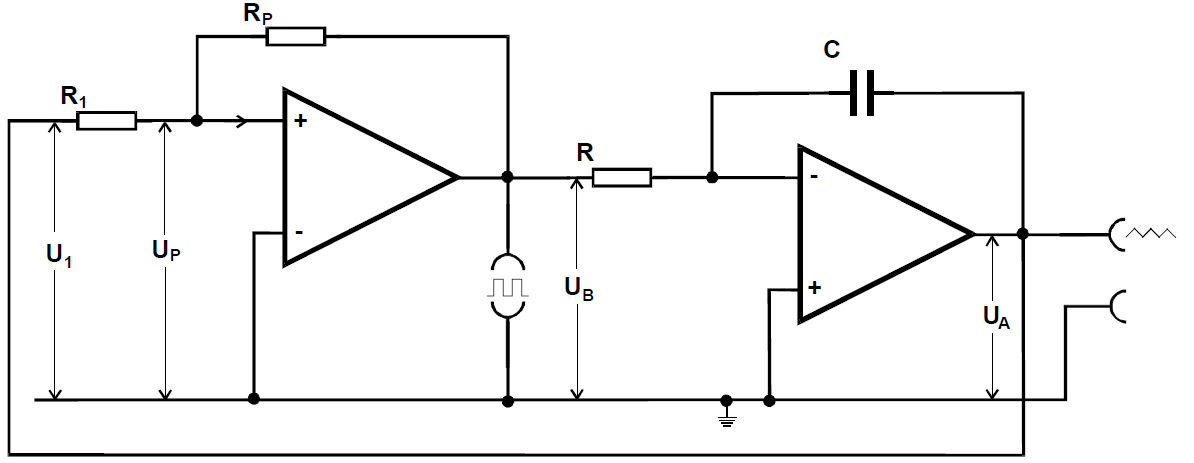
\includegraphics[width=13.0cm]{images/schaltplan_generator.png}
\caption{Schaltplan eines Rechteck-/Dreieckgenerators. [1]}
\label{fig:schalplan_generator}
\end{figure}

\subsubsection{Erzeugung amplitudenmodulierter Sinusschwingung}
Eine Sinusschwingung mit sich zeitlich veränderlicher Amplitude lässt sich durch zwei Integratoren und einem Umkehrverstärker realisieren, wie in Abbildung \ref{fig:schalplan_schwingung} dargestellt.
Die Schaltung kann durch die Differentialgleichung
\begin{align}
\frac{d^2 U_\text{A}}{dt^2}-\frac{\eta}{10 RC} \frac{d U_\text{A}}{dt}+\frac{U_\text{A}}{R^2C^2}=0
\end{align}
beschrieben werden. Die Lösung 
\begin{align}
U_\text{A}\left(t\right)=U_0\exp \left(\frac{\eta t}{20 RC}\right)\sin \frac{t}{RC}
\end{align}
beschreibt eine gedämpfte ($\eta < 0$) bzw. entdämpfte Sinusschwingung. Dabei ist die Schwingungsdauer
\begin{align}
T=2\pi RC
\end{align}
und die Abklingdauer
\begin{align}
\tau=\frac{20RC}{\left|\eta \right| }\hspace{0.3cm}\text{.}
\end{align}
\begin{figure}[H]
\centering
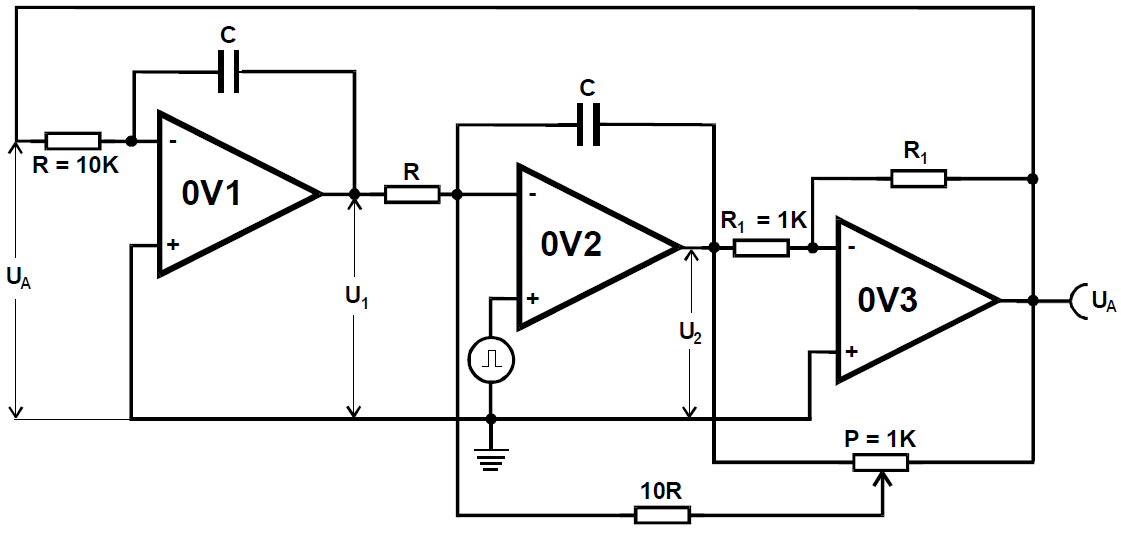
\includegraphics[width=13cm]{images/schaltplan_schwingung.png}
\caption{Schaltplan einer linearen Schwingungsdifferentialgleichung mit zeitlich veränderlichen Amplitude. [1]}
\label{fig:schalplan_schwingung}
\end{figure}
\subsubsection{Logarithmierer und Exponentialgenerator}
Ein Signal proportional zum Logarithmus oder zur Exponentialfunktion kann mit Hilfe eines Bauelement mit exponentieller Kennlinie bewerkstelligt werden, wie in Abbildung \ref{fig:schalplan_explog} dargestellt.

Ein geeignetes Bauteil ist beispielsweise eine Diode bei hinreichend großer Spannung $U$, denn dann gilt
\begin{align}
I=I_0 \exp \left(\frac{e_0}{k_\text{B} T}U\right)
\end{align}
mit der Elementarladung $e_0$, der Boltzmann-Konstante $k_\text{B}$ und der Temperatur $T$. 


\begin{figure}[H]
\centering
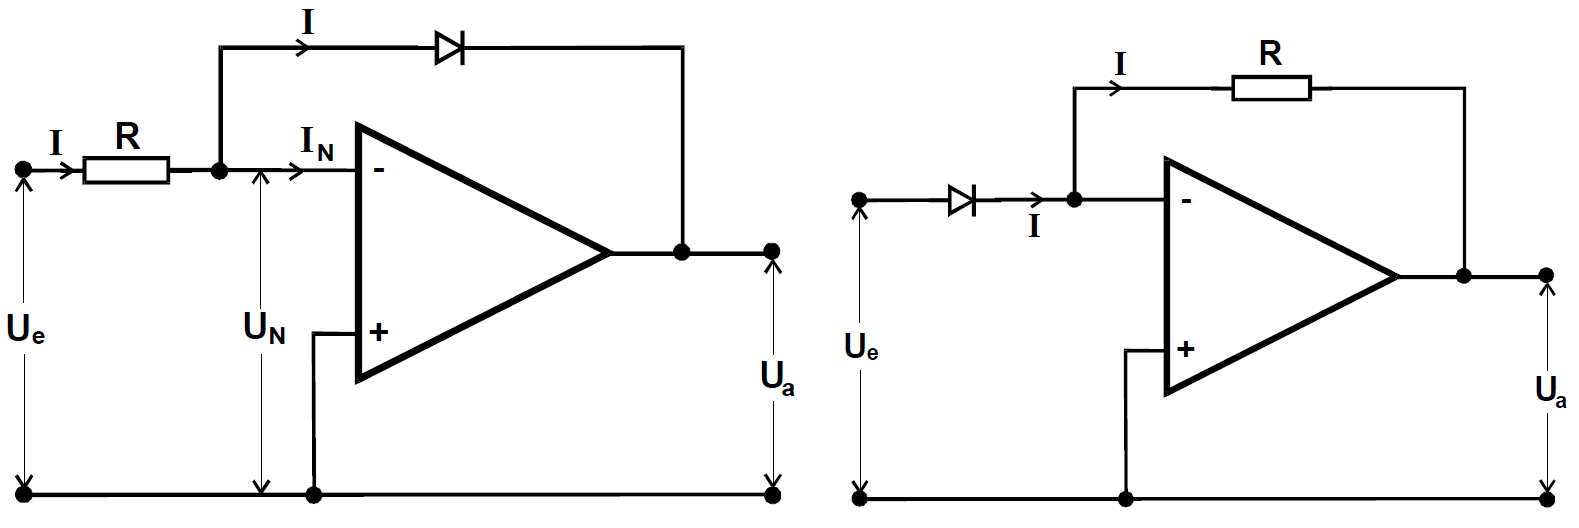
\includegraphics[width=15cm]{images/schaltplan_explog.png}
\caption{Schaltplan eines Logarithmierer (links) und eines Exponentialgenerator (rechts). [1]}
\label{fig:schalplan_explog}
\end{figure}

Es ergibt sich für einen Logarithmierer die Ausgangsspannung 
\begin{align}
U_\text{A}=\frac{k_\text{B}T}{e_0}\ln \left(\frac{U_\text{e}}{I_0 R}\right)
\end{align}
und für einen Exponentialgenerator die Ausgangsspannung
\begin{align}
U_\text{A}=RI_0\exp \left(\frac{e_0}{k_\text{B} T}U_\text{e}\right)\hspace{0.3cm}\text{.}
\end{align}

\newpage

\section{Durchführung}

\subsection{Frequenzgang des gegengekoppelten Verstärkers}
Ein gegengekoppelter Verstärker wird aufgebaut und bei vier verschiedenen Verstärkungen V' wird der entsprechende Frequenzgang vermessen.

\subsection{Der Umkehrintegrator}
Ein Umkehrintegrator wird aufgebaut und die Beziehung $U_A\propto\frac{1}{\omega}$ überprüft. Außerdem werden eine Sinus-, eine Rechteck- und eine Dreiecksspannung auf den Umkehrintegrator gegeben und von den Ausgangssignalen Bilder erstellt.

\subsection{Der Umkehrdifferentiator}
Es wird ein Umkehrdifferentiator aufgebaut und der Zusammenhang zwischen Ausgangsspannung $U_A $ und $\omega$ untersucht. Außerdem werden wieder Bilder von den Ausgangssignalen bei den oben genannten Spannungsformen aufgenommen.

\subsection{Der Schmitt-Trigger}
Ein Schmitt-Trigger wird aufgebaut und der Scheitelwert der Spannung sowie die Betriebsspannung gemessen.

\subsection{Der Dreiecksgenerator}
Ein Dreieckgenerator wird aufgebaut und ein Bild der erzeugten Spannung aufgenommen. Desweiteren werden Amplitude und Frequenz des Ausgangssignals ermittelt.

\subsection{Die Schwingungsdifferentialschaltung}
Mithilfe einer Schwingungsdifferentialschaltung wird eine ungedämpfte und eine gedämpfte Sinusspannung erzeugt. Davon werden Bilder aufgenommen und die Abklingdauer der gedämpften Schwingung bestimmt.

\subsection{Phasenbeziehung des gegengekoppelten Verstärkers}
Die Phasenbeziehung zwischen Ausgangs- und Eingangsspannung wird bei einer Verstärkung V' bestimmt.

\section{Auswertung}

\subsection{Frequenzgang des gegengekoppelten Verstärkers}

In den Abbildungen \ref{fig:freq1}-\ref{fig:freq4} sind die Frequenzgänge des gegengekoppelten Verstärkers für verschiedene Verstärkungsgrade $V'$ dargestellt. Es wurde dabei stets ein Widerstand der Größe $R_1=\SI{1}{\kilo\ohm}$ verwendet. \\
\begin{minipage}[t]{0.5\textwidth}
	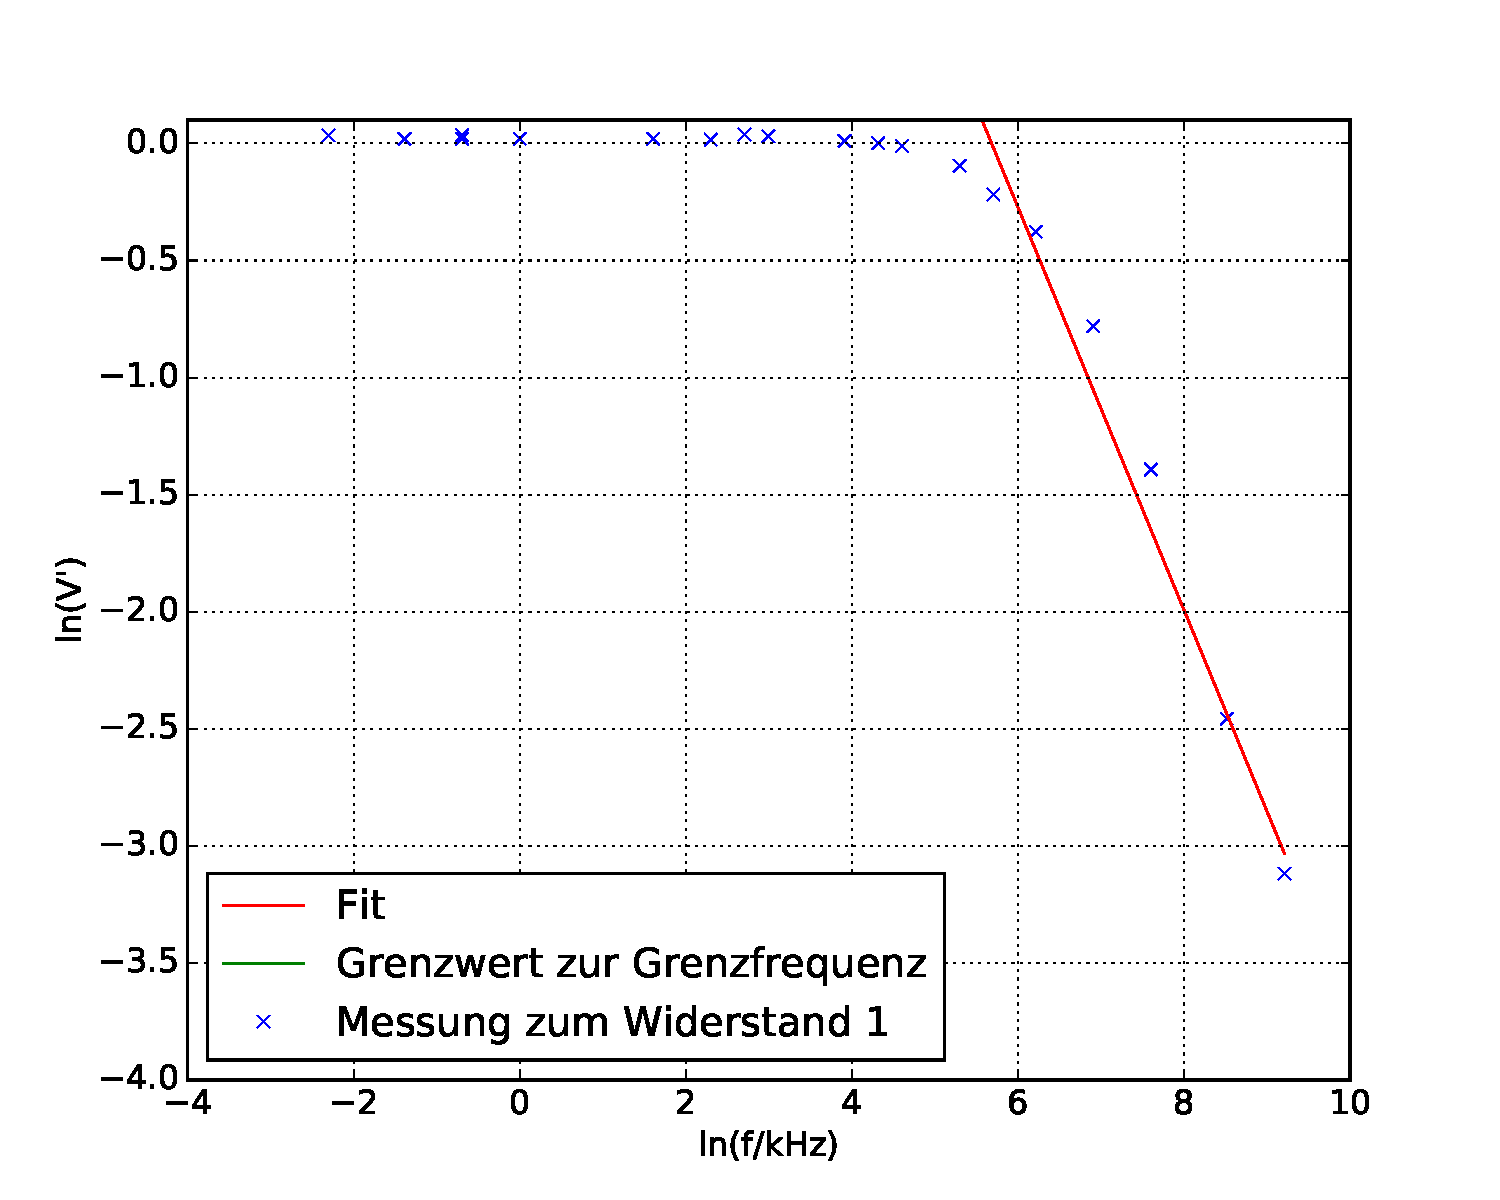
\includegraphics[width=\textwidth]{images/plot1.pdf}
	\captionof{figure}{Frequenzgang für R$_n=\SI{1}{\kilo\ohm}$}
	\label{fig:freq1}
\end{minipage}
\begin{minipage}[t]{0.5\textwidth}
	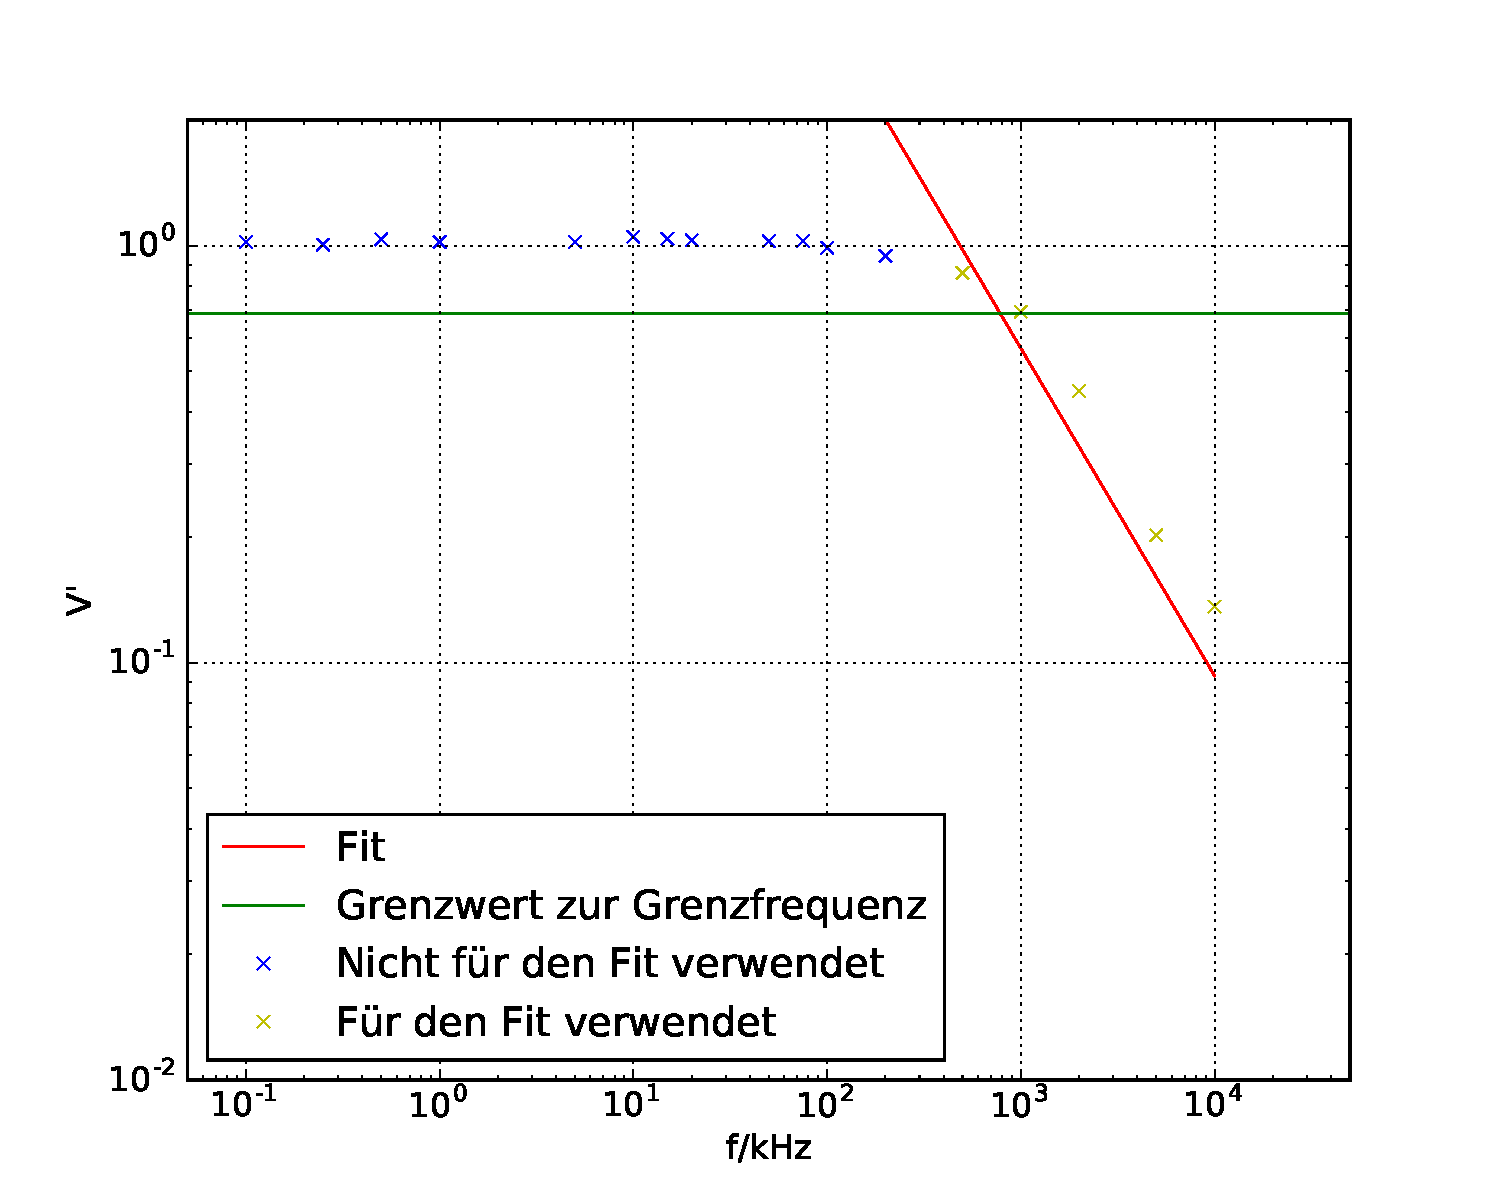
\includegraphics[width=\textwidth]{images/plot2.pdf}
	\captionof{figure}{Frequenzgang für R$_n=\SI{100}{\ohm}$}
\end{minipage} \\
\begin{minipage}[t]{0.5\textwidth}
	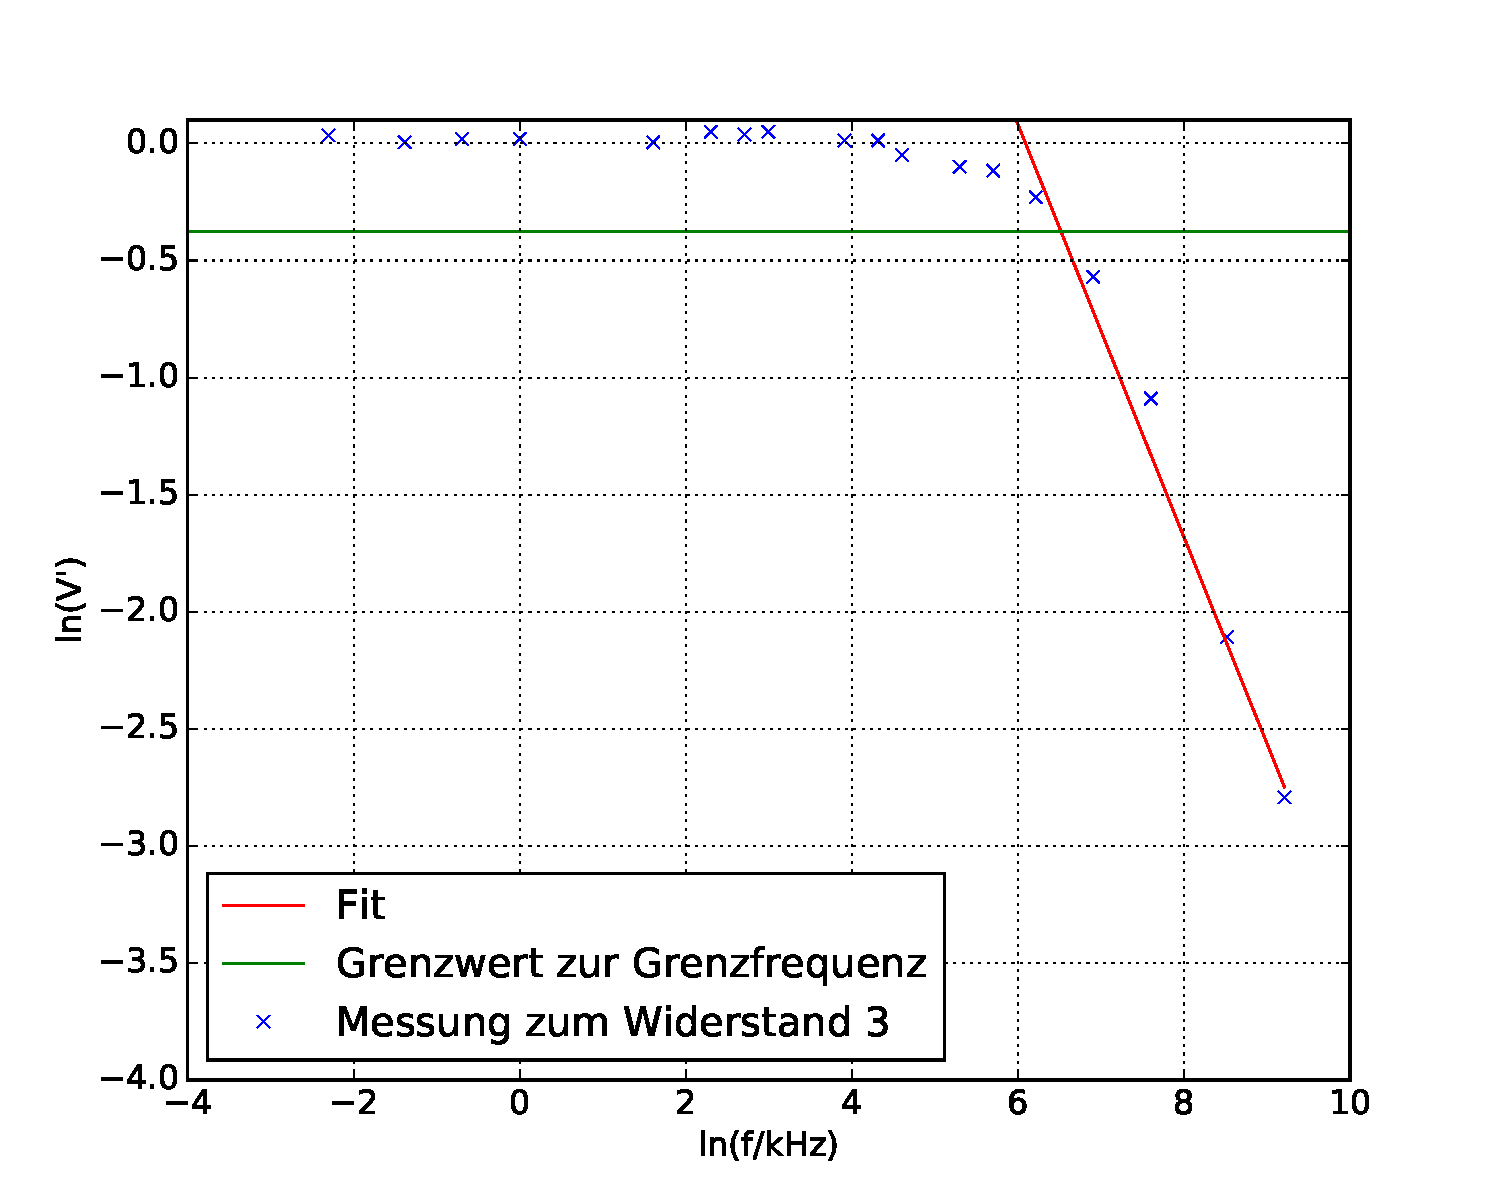
\includegraphics[width=\textwidth]{images/plot3.pdf}
	\captionof{figure}{Frequenzgang für R$_n=\SI{570}{\ohm}$}
\end{minipage}
\begin{minipage}[t]{0.5\textwidth}
	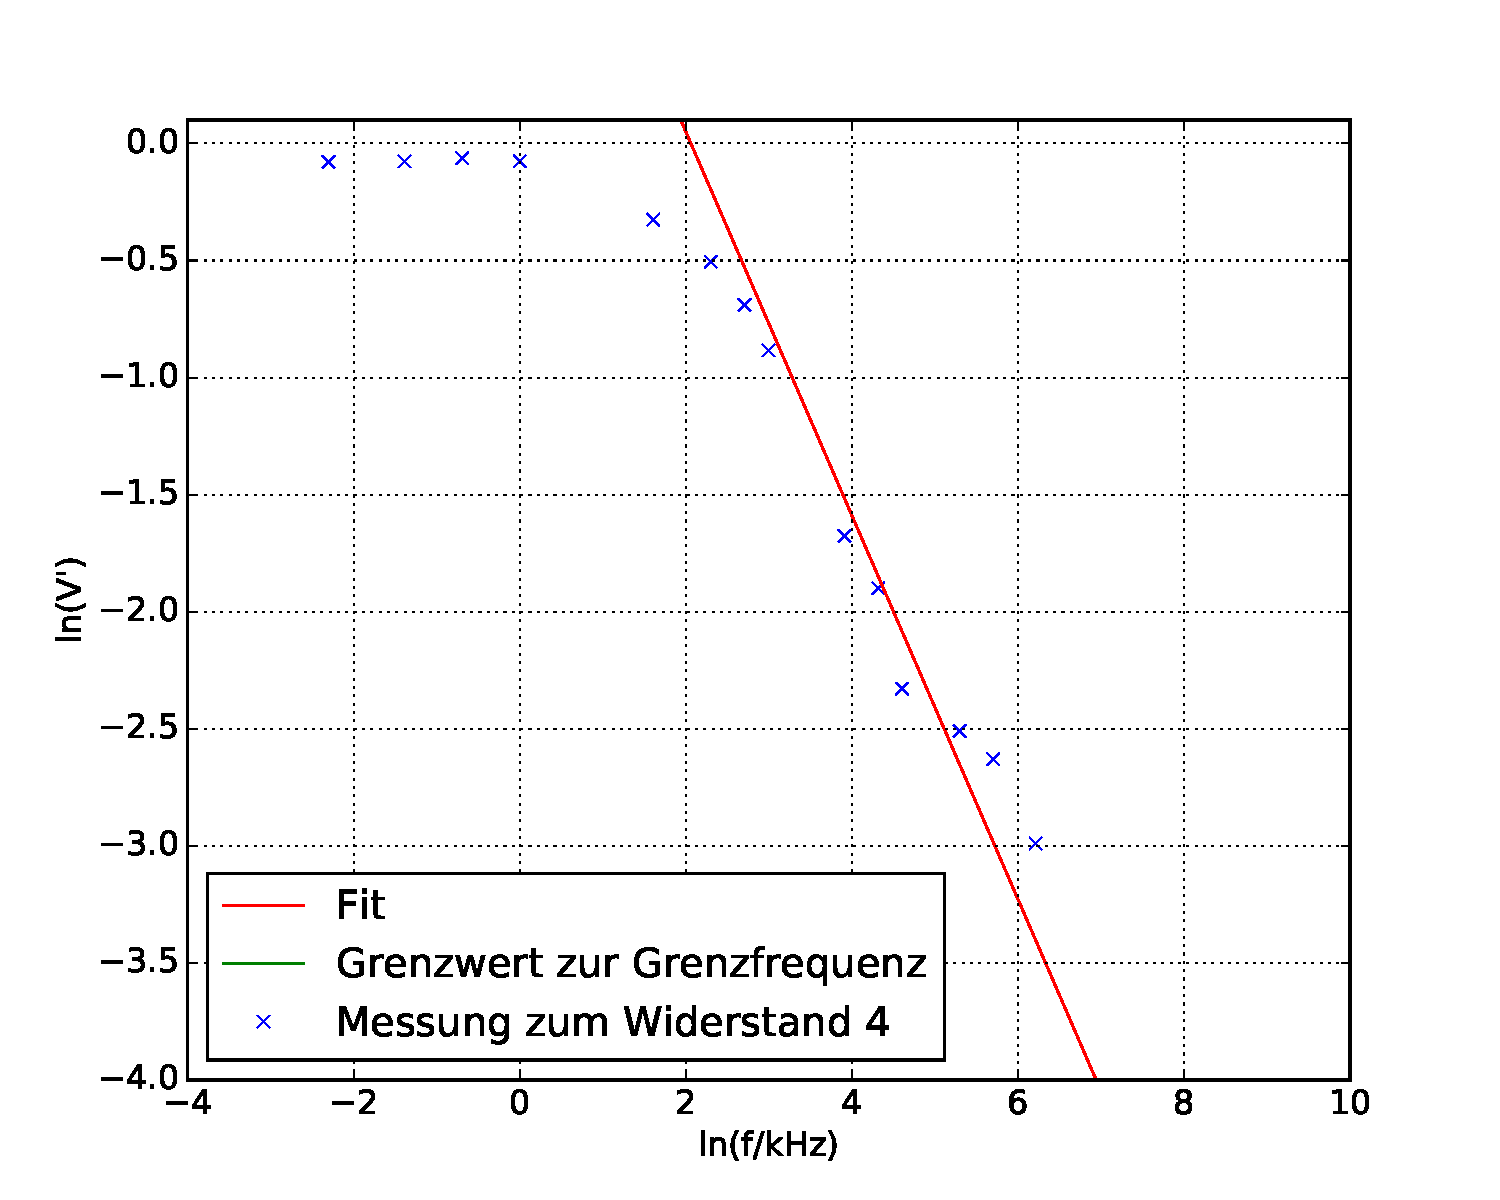
\includegraphics[width=\textwidth]{images/plot4.pdf}
	\captionof{figure}{Frequenzgang für R$_n=\SI{100}{\kilo\ohm}$}
	\label{fig:freq4}
\end{minipage} \\
\\
In Tabelle \ref{tab:frequenzgang} sind die Grenzfrequenz, die Verstärkung in Theorie und Experiment, die Leerlaufverstärkung, die Steigung m und das Verstärkungs-Bandbreite-Produkt für die einzelnen verwendeten Widerstände dargestellt. \\
\begin{table}[H]
		\captionof{table}{Experimentell bestimmte Kenndaten}
		\label{tab:frequenzgang}
		\hskip-1.50cm\begin{tabular}{r r r r r}
			\toprule
				Kenngröße & $R_n=\SI{1}{\kilo\ohm}$ & $R_n=\SI{100}{\ohm}$ &  $R_n=\SI{570}{\ohm}$ & $R_n=\SI{100}{\kilo\ohm}$ \\
			\midrule
				Grenzfrequenz f [kHz] & $450 \pm 350$ & $1000 \pm 500$ & $700 \pm 500$ & $14 \pm 11$ \\
				$V'_{ideal}$ & $1.0$ & $0.1$ & $0.57$ & $100$ \\
				$V'_{exp}$ & $0.980 \pm 0.007$ & $0.970 \pm 0.012$ & $0.970 \pm 0.012$ & $0.884 \pm 0.006$ \\
				$V_{Leerlauf}$ & $48.25 \pm 17.04$ & $-0.111 \pm 0.000$ & $-1.38 \pm 0.02$ & $0.892 \pm 0.006$ \\
				Steigung m & $-0.860 \pm 0.070$ & $-0.897 \pm 0.046$ & $-0.882 \pm 0.070$ & $-0.819 \pm 0.098$\\
				Verstärkung-Bandbreite-Produkt [kHz] & $441.58 \pm 347.37$ & $955.89 \pm 525.67$ & $658.61 \pm 529.53$ & $12.33 \pm 9.51$ \\
			\bottomrule
		\end{tabular}
\end{table}
Die Abnahme des Ausgangsamplitude ist damit zu erklären, dass der gekoppelte Verstärker, wie in Abbildung \ref{fig:tiefpass} dargestellt, die Funktion eines Tiefpasses hat.
\begin{center}
	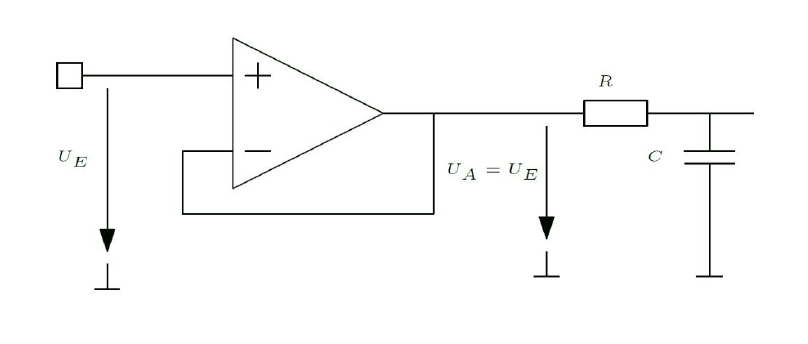
\includegraphics[width=10cm]{images/tiefpass.png}
	\captionof{figure}{Ersatzschaltbild des Tiefpasses}
	\label{fig:tiefpass}
\end{center}

\subsection{Der Umkehrintegrator}
Für den Aufbau des Umkehrintegrators wurden ein Widerstand $R=\SI{32.7}{\kilo\ohm}$ und eine Kapazität $C=\SI{13.6}{\nano\farad}$ verwendet. Die gemessenen Ausgangsspannungen in Abhängigkeit von der Frequenz sind in Tabelle \ref{tab:integrator} dargestellt, in Abbildungen \ref{fig:sinusint}-\ref{fig:dreieckint} sind die Thermodrucke des Ausgangssignals für verschiedene Eingangssignalformen dargestellt.
\begin{table}[H]
	\centering
	\captionof{table}{Werte der Ausgangsspannung des Umkehrintegrators}
	\label{tab:integrator}
	\hskip-1.50cm
	\begin{tabular}{r r}
		\toprule
			Frequenz $f / \si{\kilo\hertz}$ & $U_A / \si{\volt}$ \\
		\midrule
			10000 & 0.19 \\
			7500  & 0.27 \\
			5000  & 0.38 \\
			2500  & 0.76 \\
			1000  & 1.49 \\
			900   & 1.57 \\
			800   & 1.65 \\
			700   & 1.73 \\
			600   & 1.81 \\
			500   & 1.87 \\
			400   & 2.01 \\
			300   & 1.75 \\
			200   & 1.69 \\
			100   & 2.41 \\
			50    & 2.41 \\
		 \bottomrule
	\end{tabular}
\end{table}
Mithilfe einer linearen Ausgleichsrechnung und einer Ausgleichsgeraden der Form $f(x)=m\cdot x +b$ ergibt sich die Steigung $m$ zu
\begin{align*}
m = -0.754\pm 0.040\,.
\end{align*}
\begin{center}
	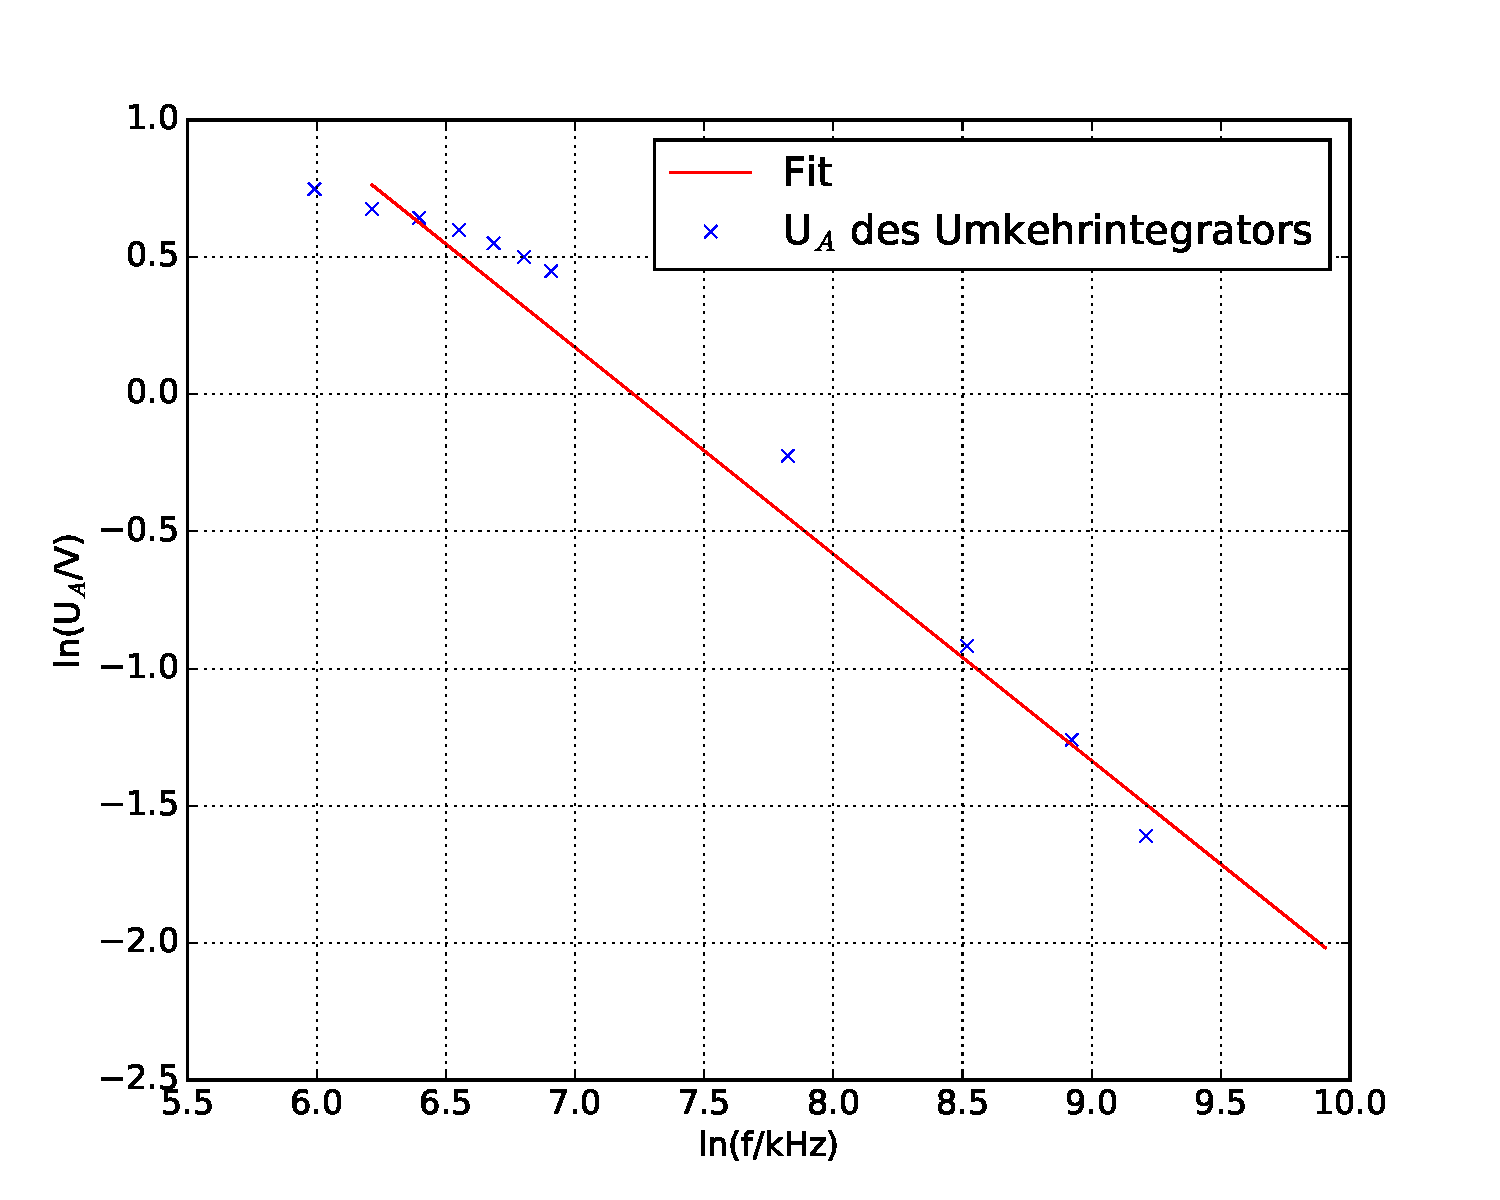
\includegraphics[width=12cm]{images/integrator.pdf}
	\captionof{figure}{Ausgangsspannung $U_A$ des Umkehrintegrators bei variierter Frequenz}
	\label{fig:integrator}
\end{center}
\begin{minipage}[t]{0.5\textwidth}
	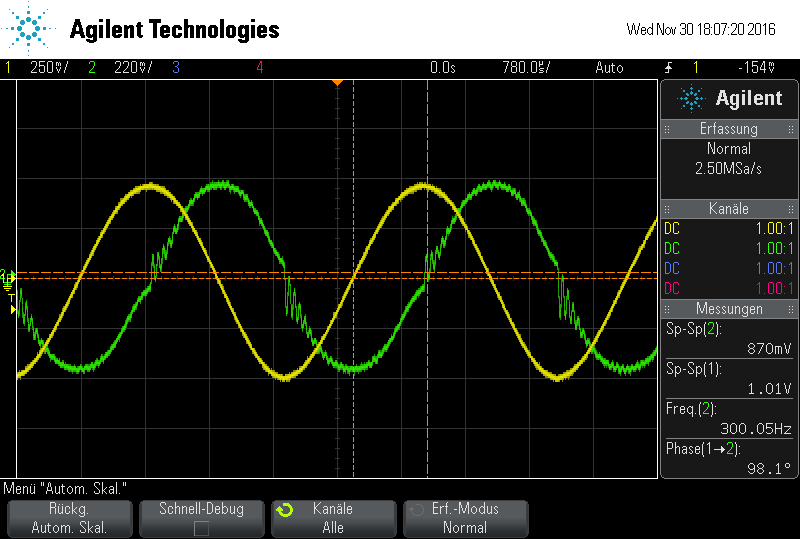
\includegraphics[width=\textwidth]{images/sinus_int}
	\captionof{figure}{Thermodruck des Signalverlaufes bei einer Sinus-Spannung}
	\label{fig:sinusint}
\end{minipage}
\hspace{0.1\textwidth}
\begin{minipage}[t]{0.5\textwidth}
	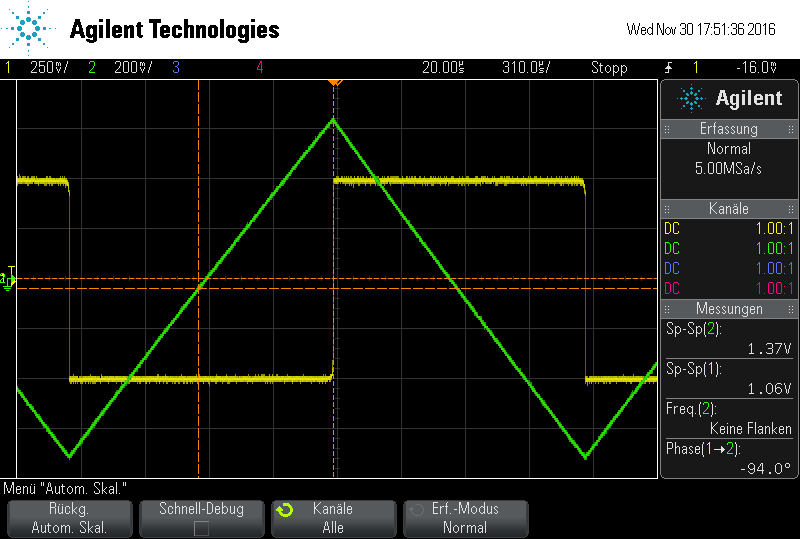
\includegraphics[width=\textwidth]{images/rechteck_int}
	\captionof{figure}{Thermodruck des Signalverlaufes bei einer Rechteck-Spannung}
	\label{fig:rechteckint}
\end{minipage} \\
\begin{minipage}[t]{0.5\textwidth}
	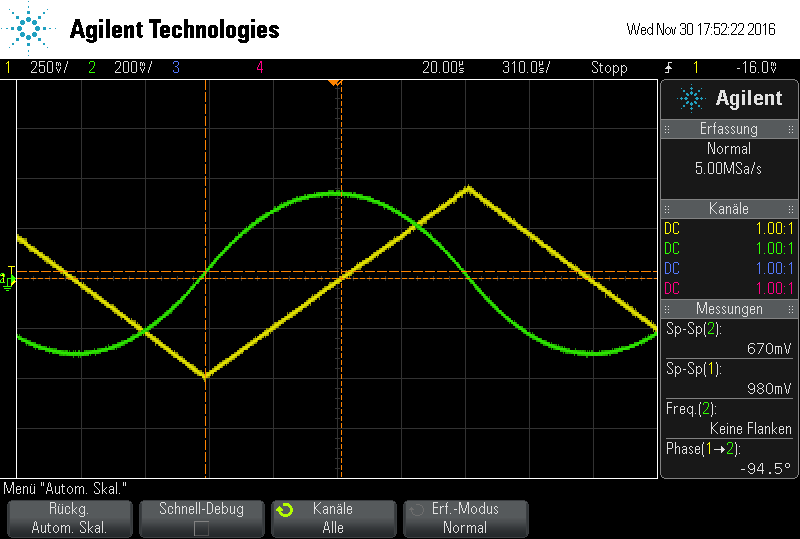
\includegraphics[width=\textwidth]{images/dreieck_int}
	\captionof{figure}{Thermodruck des Signalverlaufes bei einer Dreieck-Spannung}
	\label{fig:dreieckint}
\end{minipage}

\subsection{Der Umkehrdifferentiator}
Für den Aufbau des Umkehrdifferentiators wurden ein Widerstand $R=\SI{32.7}{\kilo\ohm}$ und eine Kapazität $C=\SI{13.6}{\nano\farad}$ verwendet. Die gemessenen Ausgangsspannungen in Abhängigkeit von der Frequenz sind in Tabelle \ref{tab:differentiator} dargestellt, in Abbildungen \ref{fig:sinusdiff}-\ref{fig:dreieckdiff} sind die Thermodrucke des Ausgangssignals für verschiedene Eingangssignalformen dargestellt.
\begin{table}[H]
	\centering
	\captionof{table}{Werte der Ausgangsspannung des Umkehrdifferentiators}
	\label{tab:differentiator}
	\hskip-1.50cm
	\begin{tabular}{r r}
		\toprule
		Frequenz $f / \si{\kilo\hertz}$ & $U_A / \si{\volt}$ \\
		\midrule
		10000 & 0.18 \\
		7500  & 0.27 \\
		5000  & 0.40 \\
		2500  & 0.77 \\
		1000  & 1.45 \\
		900   & 1.53 \\
		800   & 1.59 \\
		700   & 1.67 \\
		600   & 1.73 \\
		500   & 1.79 \\
		400   & 1.75 \\
		300   & 1.61 \\
		200   & 1.55 \\
		100   & 1.51 \\
		50    & 1.49 \\
		\bottomrule
	\end{tabular}
\end{table}
Mithilfe einer linearen Ausgleichsrechnung und einer Ausgleichsgeraden der Form $f(x)=m\cdot x +b$ ergibt sich die Steigung $m$ zu
\begin{align*}
m = -0.797 \pm 0.039\,.
\end{align*}
\begin{center}
	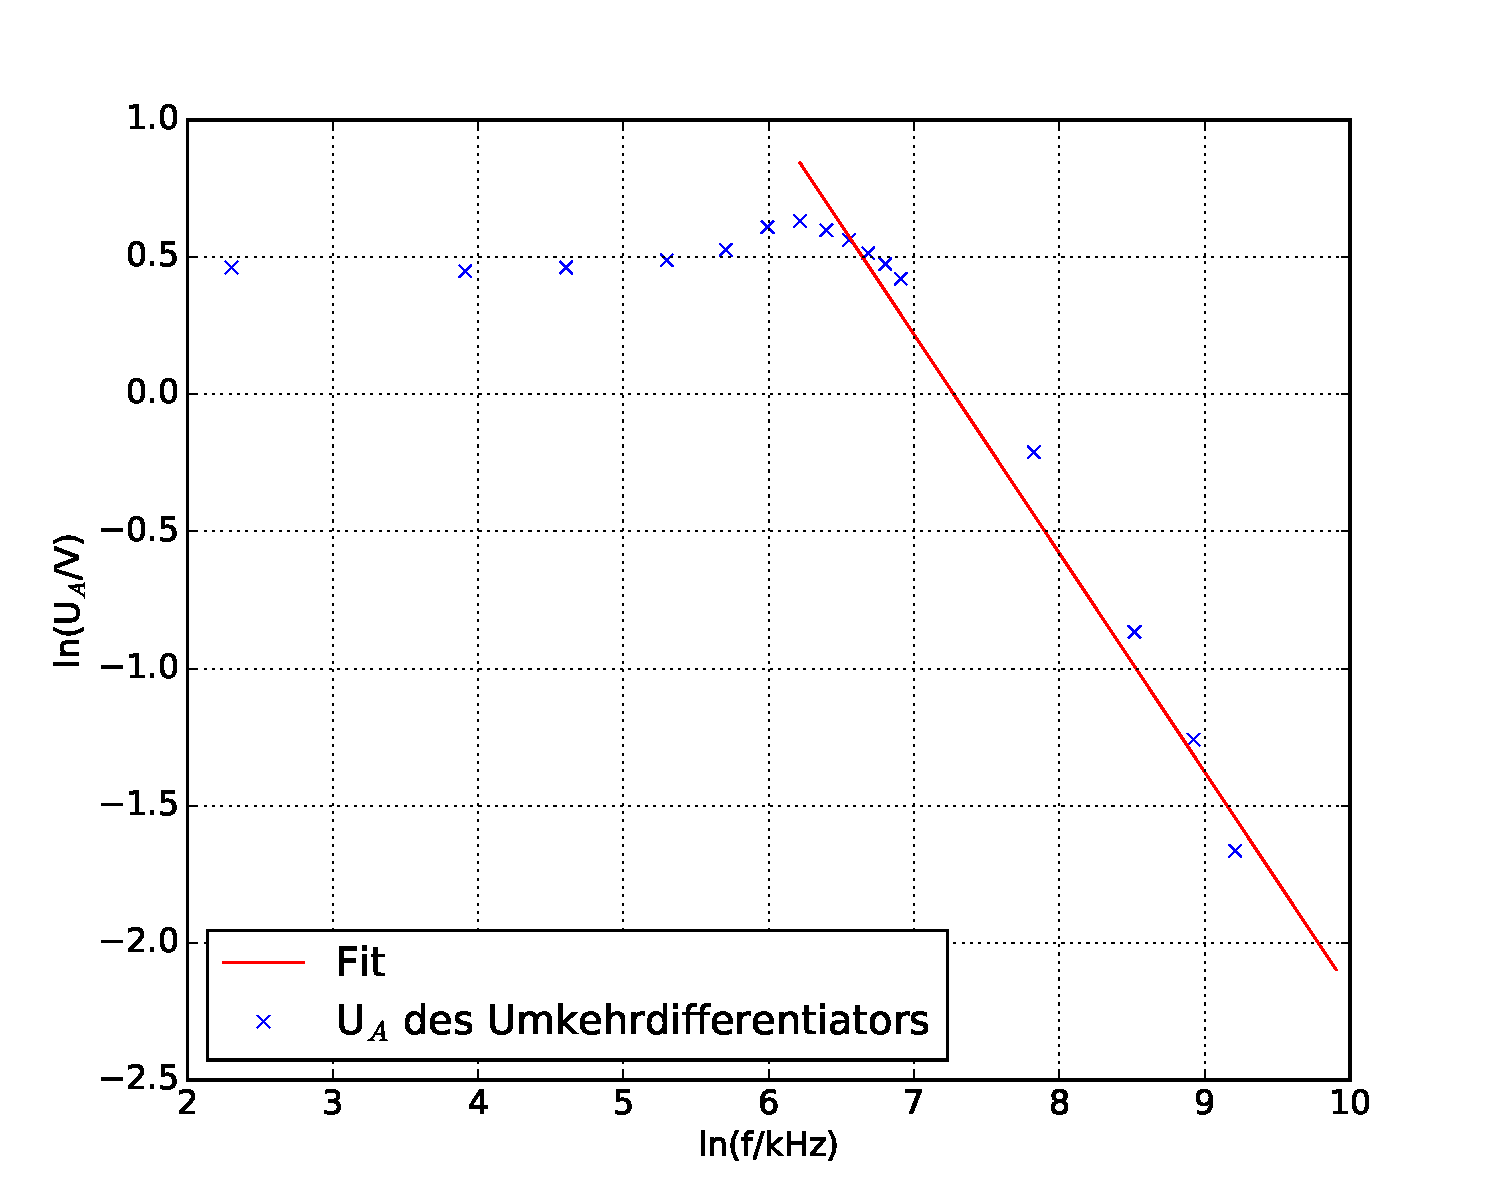
\includegraphics[width=12cm]{images/differentiator.pdf}
	\captionof{figure}{Ausgangsspannung $U_A$ des Umkehrdifferentiators bei variierter Frequenz}
	\label{fig:differentiator}
\end{center}
\begin{minipage}[t]{0.5\textwidth}
	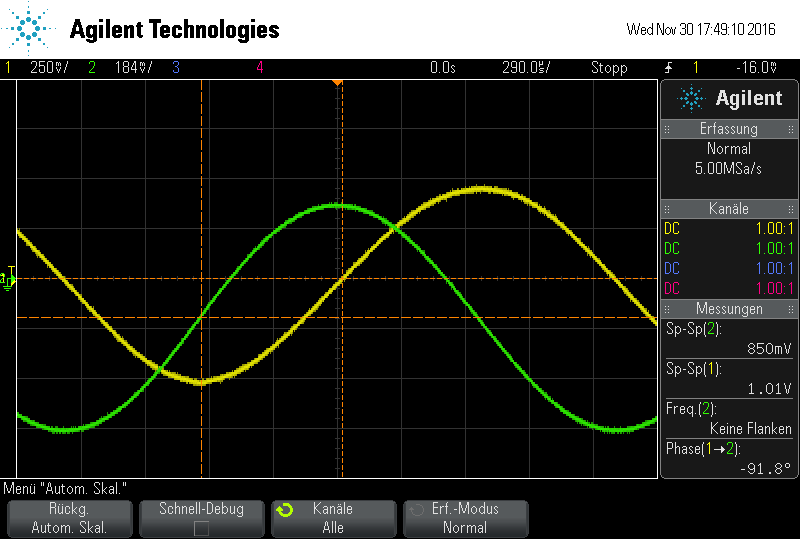
\includegraphics[width=\textwidth]{images/sinus_diff}
	\captionof{figure}{Thermodruck des Signalverlaufes bei einer Sinus-Spannung}
	\label{fig:sinusdiff}
\end{minipage}
\hspace{0.1\textwidth}
\begin{minipage}[t]{0.5\textwidth}
	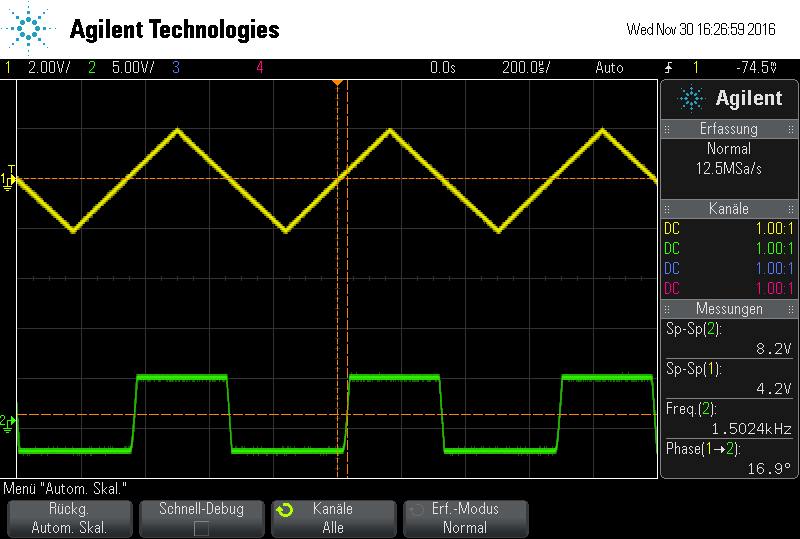
\includegraphics[width=\textwidth]{images/rechteck_diff}
	\captionof{figure}{Thermodruck des Signalverlaufes bei einer Rechteck-Spannung}
	\label{fig:rechteckdiff}
\end{minipage} \\
\begin{minipage}[t]{0.5\textwidth}
	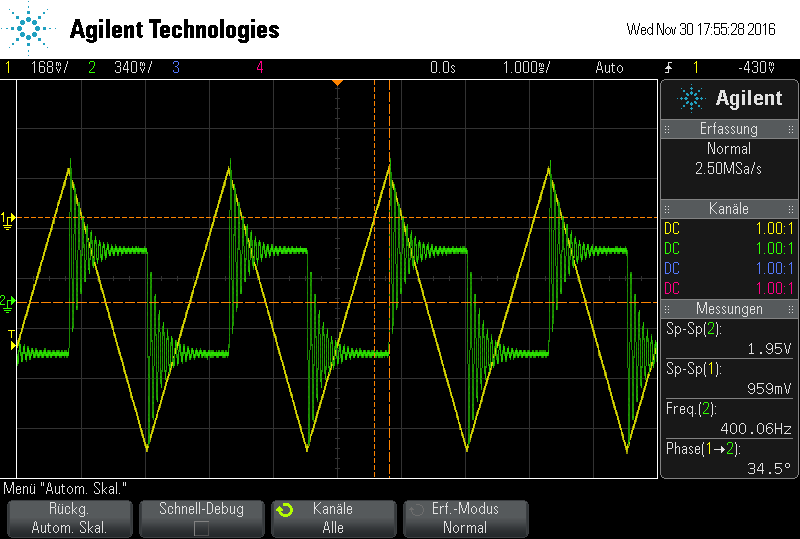
\includegraphics[width=\textwidth]{images/dreieck_diff}
	\captionof{figure}{Thermodruck des Signalverlaufes bei einer Dreieck-Spannung}
	\label{fig:dreieckdiff}
\end{minipage} 

\subsection{Der Schmitt-Trigger}
Für den Aufbau des Schmitt-Triggers wurden die Widerstände $R_P=\SI{33}{\kilo\ohm}$ und $R_1=\SI{100}{\ohm}$ verwendet. Der Wert des Betriebsspannung betrug $U_B=\SI{13.08}{\volt}$. \\
Der Kippspannung betrug $U_{kipp}=\SI{90}{\milli\volt}$ die theoretisch errechnete Kippspannung betrug
\begin{align*}
U_{theor}=\SI{39.6}{\milli\volt}\,.
\end{align*}

\subsection{Der Dreiecksgenerator}
Der Dreieckgenerator wurde mit der Konfiguration
\begin{align*}
R_1=\SI{100}{\ohm} && R_P=\SI{33}{\kilo\ohm} && R=\SI{10}{\kilo\ohm} && C=\SI{100}{\nano\farad}
\end{align*}
aufgebaut. \\
Die theoretische Frequenz des Dreiecksgenerators ergibt sich aus
\begin{align}
f_{theo}=\frac{R_P}{4R_1RC}\,.
\end{align}
Somit ergaben sich für diese Konfiguration folgende Werte:
\begin{align}
f_{theo}=\SI{82.5}{\kilo\hertz} &  & f_{exp}=\SI{91.34}{\kilo\hertz}\,.
\end{align}

\subsection{Die Schwingungsdifferentialschaltung}
Für die Kapazität in der Schwingungsdifferentialschaltung wurde $C=\SI{22.5}{\nano\farad}$ gewählt. \\
Die theoretischen Werte für die Frequenz $f_{theo}$ und die Abklingdauer $\tau$ ergeben sich zu
\begin{align}
f_{theo} = \frac{1}{2\pi RC}=\SI{723.43}{\hertz} \\
\tau = 20RC=\SI{4.5}{\milli\second}\,.
\end{align}
In Abbildung \ref{fig:thermoexpon_ung} ist die ungedämpfte Schwingung dargestellt, die Frequenz der Schwingung beträgt $\SI{664.2}{\hertz}$.
\begin{center}
	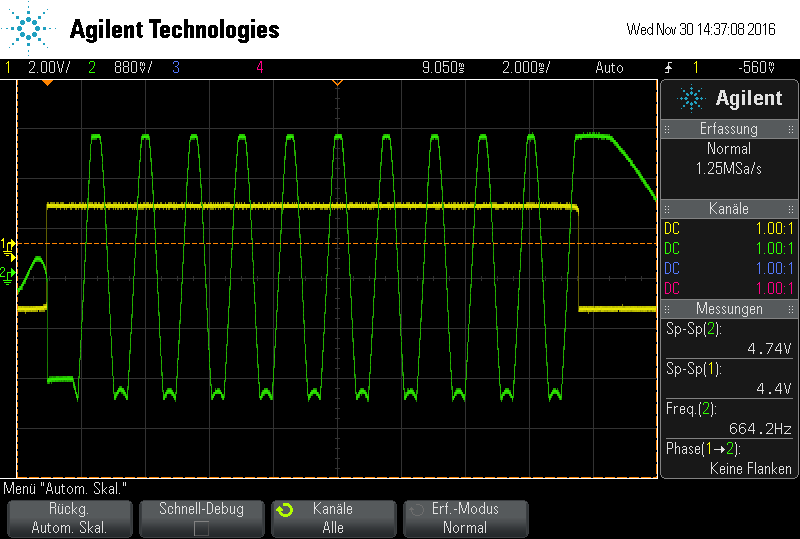
\includegraphics[width=10cm]{images/schwingung.png}
	\captionof{figure}{Thermodruck der ungedämpften Schwingung nach Anregung durch Rechteckschwingung}
	\label{fig:thermoexpon_ung}
\end{center}
Zur Bestimmung der Abklingdauer der gedämpften Schwingung werden mithilfe eines Peak-Detection-Algorithmus die Maxima bestimmt und mit diesen mit einem Exponentialansatz $f(t)=a\exp\left(-t/\tau\right) $ eine Ausgleichsrechnung durchgeführt. In Abbildung \ref{fig:expfit} sind der nicht-lineare Fit sowie die Messwerte dargestellt, ein Thermodruck des Oszilloskopenbildes ist in Abbildung \ref{fig:thermoexpon} dargestellt. \\
Aus der nicht-linearen Ausgleichsrechnung ergibt sich die Abklingdauer von
\begin{align*}
\tau_{exp}=\SI{4.1(2)}{\milli\second}\,.
\end{align*}
\begin{center}
	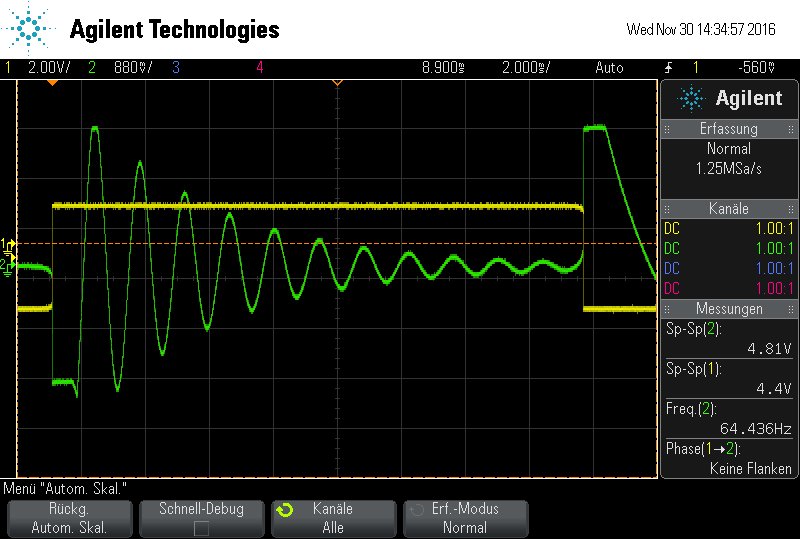
\includegraphics[width=10cm]{images/schwinggen.png}
	\captionof{figure}{Thermodruck des exponentiellen Abfalls nach Anregung durch Rechteckschwingung}
	\label{fig:thermoexpon}
\end{center}
\begin{center}
	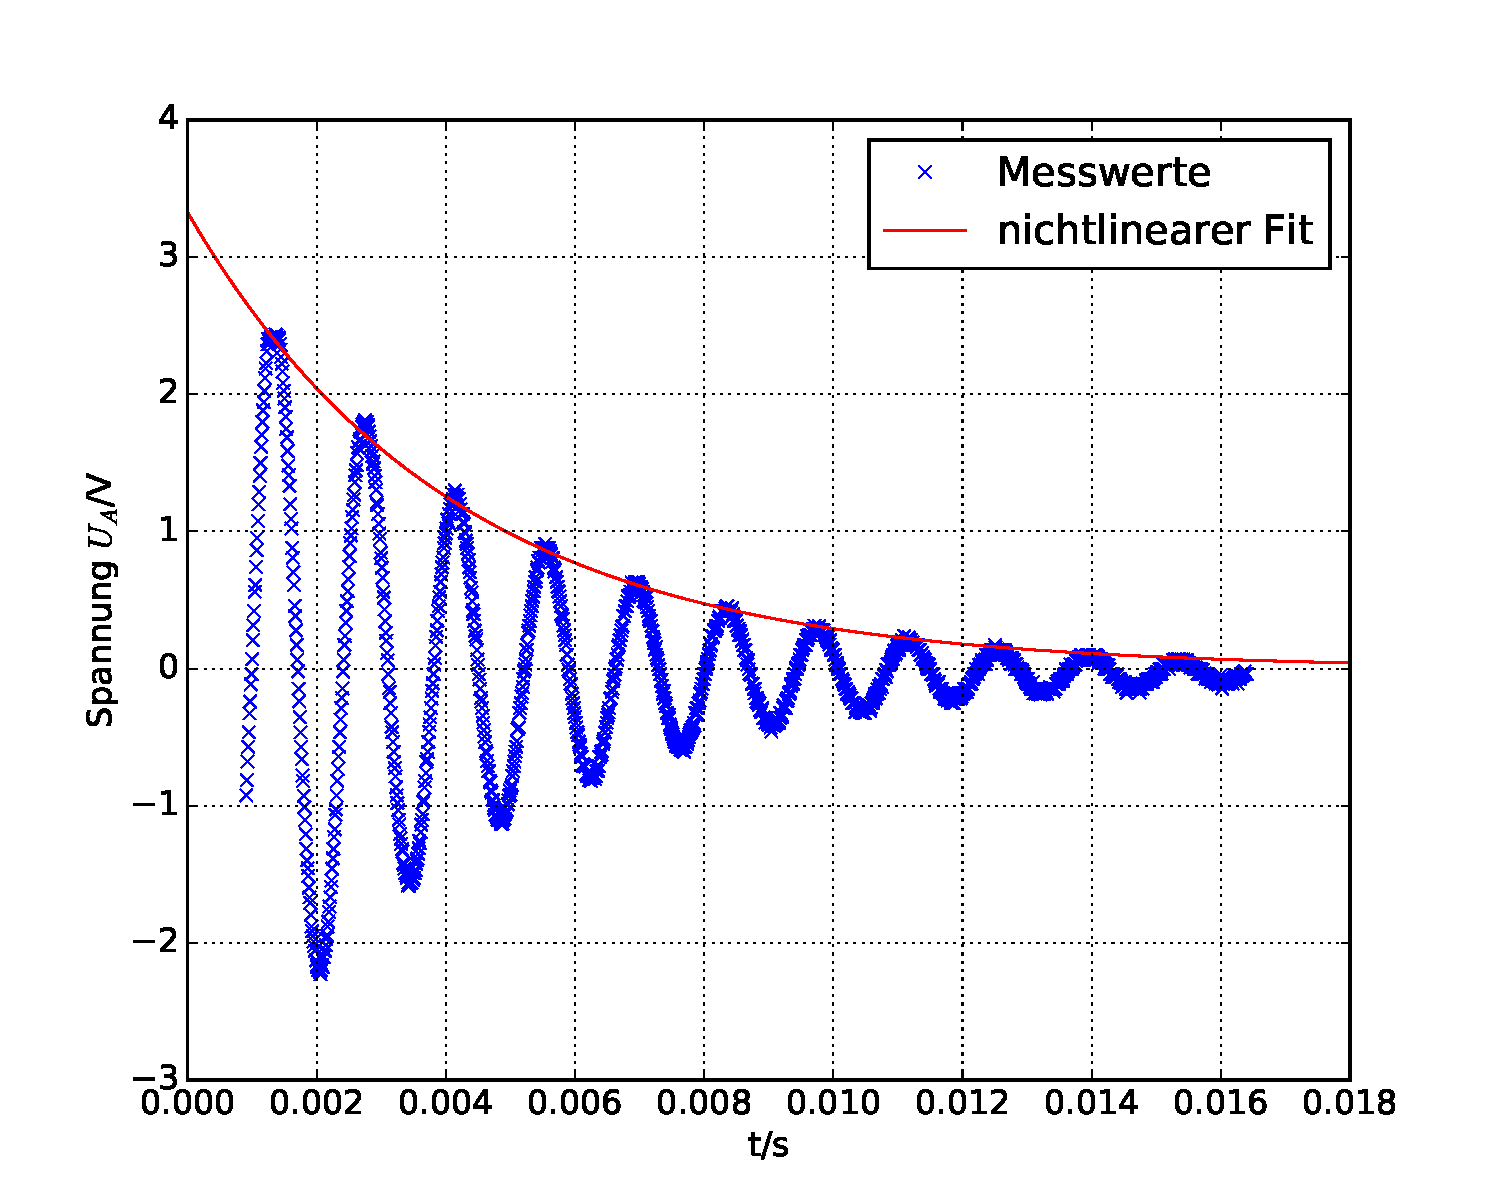
\includegraphics[width=10cm]{images/schwing_abfall.pdf}
	\captionof{figure}{Messwerte zum Schwingabfall des Signals und nichtlinearer Fit der Maxima}
	\label{fig:expfit}
\end{center}

\subsection{Phasenbeziehung des gegengekoppelten Verstärkers}
In Abbildung \ref{fig:phase} sind die Messwerte für die Phasenverschiebung zwischen Eingangs- und Ausgangsspannung dargestellt.
\begin{center}
	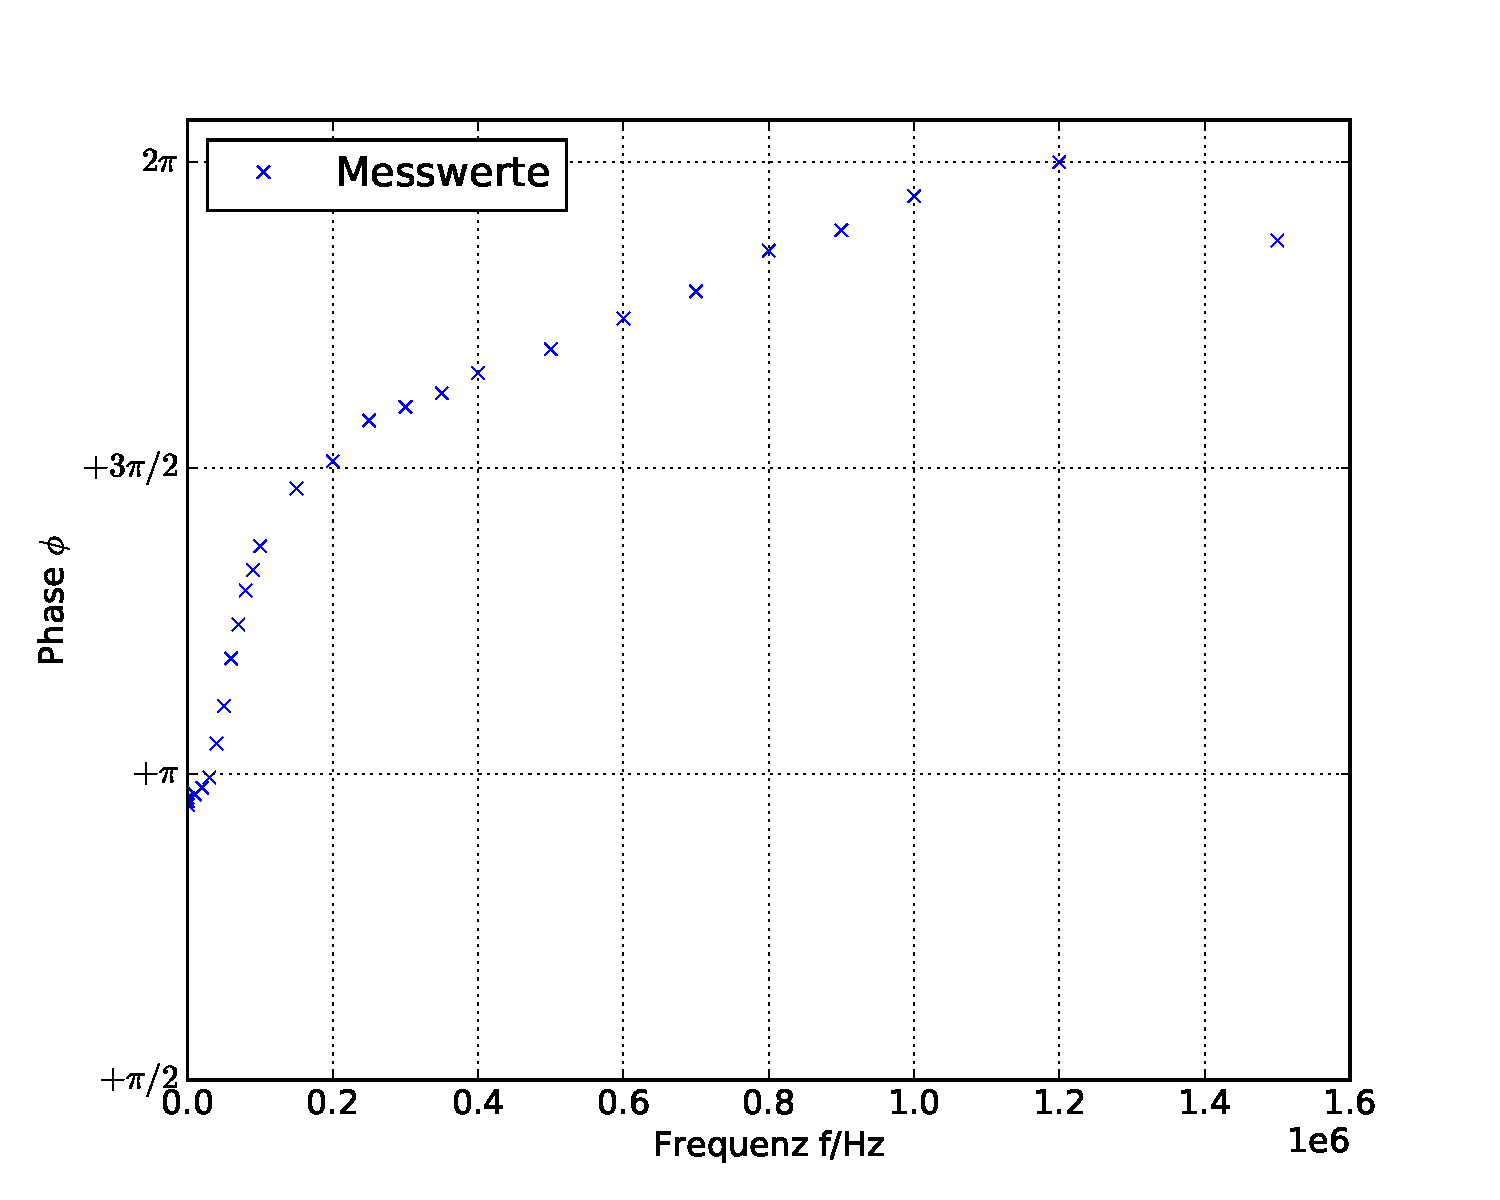
\includegraphics[width=10cm]{images/phase_frequenz.pdf}
	\captionof{figure}{Phasenverschiebung zwischen Eingangs- und Ausgangsspannung aufgetragen gegen die Fequenz}
	\label{fig:phase}
\end{center}

\section{Diskussion}

\subsection{Frequenzgang des gegengekoppelten Verstärkers}
Die experimentell bestimmten Verstärkungen liegen nur im Falle von $R_n=\SI{1}{\kilo\ohm}$ und bei $R_n=\SI{570}{\ohm}$ mit 0.02\% und 70\% Abweichung vom Theoriewert in der gleichen Größenordnung wie der Theoriewert. \\
Desweiteren ergeben sich bei $R_n=\SI{100}{\ohm}$ und bei $R_n=\SI{570}{\ohm}$ physikalisch nicht sinnvolle negative Leerlaufverstärkungen. Das eigentlich konstante Verstärkungs-Bandbreite-Produkt ist hier auch für jeden Widerstand unterschiedlich, was jedoch aus den vorherigen Abweichungen resultiert. \\
Desweiteren ist auffällig, dass die Fehler der ermittelten Grenzfrequenzen sehr hoch sind. Dies resultiert aus dem Anwenden der Exponentialfunktion auf die ermittelten Fit-Parameter, deren Fehler noch nicht diese Größe hatte. \\
Der Theoriewert der Steigung ist m=-1 (für einen Tiefpass), die Steigungen der verschiedenen Konfigurationen schwanken zwischen -0.897 und -0.819, haben also signifikante Abweichungen vom theoretisch erwarteten Wert.

\subsection{Der Umkehrintegrator}
Der Umkehrintegrator funktioniert wie erwartet, wie an den aufgenommen Bilder der Oszilloskopausgabe zu sehen ist. Da für den Integrator die Beziehung $U_A\propto\omega^{-1}$ gelten soll, lautet der Theoriewert $m=-1$. Die lineare Regression ergab einen Wert von $m=-0.754\pm0.040$, welcher um 24.6\% vom Theoriewert abweicht.

\subsection{Der Umkehrdifferentiator}
Der Umkehrdifferentiator arbeitete, wie auf den aufgenommenen Bildern zu sehen ist, wie erwartet. Jedoch ergab sich eine starke Abweichung von der Beziehung $U_A\propto\omega$. Der theoretisch erwartete Wert für die Steigung m war m=1, jedoch ergab die lineare Regression einen Wert von $m = -0.797 \pm 0.039$. Dies lässt sich auf einen systematischen Fehler im Aufbau oder in Apparatur zurückführen.

\subsection{Der Schmitt-Trigger}
Der Schmitt-Trigger arbeitet zwar wie erwartet, die Kippspannung weicht jedoch mit 127\% signifikant vom theoretisch erwarteten Wert ab. Hier ist von einem systematischen Fehler im Aufbau oder der Apparatur auszugehen.

\subsection{Der Dreiecksgenerator}
Der Dreiecksgenerator liefert wie erwartet ein Dreieckssignal. Die experimentell bestimmte Frequenz des Dreieckgenerators weicht um 10.70\% vom berechneten Theoriewert ab.

\subsection{Die Schwingungsdifferentialschaltung}
Die Schwingungsdifferentialschaltung funktioniert, wie auf den Thermodrucken zu sehen ist, wie erwartet. Für die Frequenz der Schaltung ergibt ein experimentell bestimmter Wert von $f_{exp}=\SI{664.2}{\hertz}$, was mit 8.2\% vom Theoriewert $f_{theo}=\SI{723.43}{\hertz}$ abweicht. \\
Die Abklingdauer liegt bei $\tau_{exp}=\SI{4.1(2)}{\milli\second}$, diesec weicht um 8,9\% vom Theoriewert ab, dies liegt außerhalb des angegebenen statistischen Fehlers.

\subsection{Phasenbeziehung des gegengekoppelten Verstärkers}
In der Abbildung ist deutlich zu erkennen, dass der Absolutbetrag der Phasendifferenz zwischen Eingangs- und Ausgangsspannung mit steigender Frequenz abnimmt. 

\section{Quellen}
{[1]} Physikalisches Praktikum, TU Dortmund: \\
Versuchsanleitung zu Versuch 51: \\
http://129.217.
224.2/HOMEPAGE/PHYSIKER/MASTER/SKRIPT/V51.pdf (letzte Version vom 02.01.2017, 11:10)\\
\end{document}